\graphicspath{{./05-Numerique/images/}}

\chapter{Travaux numériques}
\label{chap:numerique}

Les travaux présentés jusqu'ici sont issus de l'expérimentation. Trois échantillons d'une poudre de polystyrène ont été soumis à des essais de compression triaxiale. La présence de capteurs de force et déplacement sur la cellule de charge rend possible l'analyse de la réponse mécanique de l'échantillon lors de l'essai. La mise en place du dispositif dans un tomographe permet en prime l'analyse de la microstructure de l'échantillon en cours de compression et donc de connaître, par l'intermédiaire de la corrélation de volumes, la cinématique au sein de l'échantillon.
\\Les travaux qui vont être présentés dans ce chapitre ont pour objectif de développer une méthode numérique qui permet d'étudier le comportement d'un ensemble de grains constituant les différents échantillons par l'intermédiaire de simulations basées sur la géométrie réelle des grains et leur mesures cinématiques.
\\Il est cependant nécessaire de lever certains verrous dans l'accomplissement de cette tâche. Il faut tout d'abord que l'identification de chaque grain puisse être faite : une méthode de segmentation est développée pour cela. Il faut ensuite transformer les images 3D des grains voxellisés en une structure d'éléments finis dont la géométrie doit rester fidèle à celle du grains numérisé. Le processus de maillage et le choix d'éléments finis sont alors optimisés. Enfin, un modèle doit être créé pour permettre au logiciel commercial Abaqus \citep{abaqus2016} de mener les simulations numériques. Ce modèle doit tenir compte de la cinématique mesurée dans l'échantillon afin de déterminer les conditions aux limites de l'échantillon numérique mais aussi établir des lois de comportement et de contact adaptées au matériau polystyrène. Pour finir, l'ensemble de ces tâches est amené à être répété de nombreuses fois afin de mener l'étude numérique sur plusieurs sous-volumes des échantillons. Un algorithme a donc été développé dans l'objectif de mener plusieurs campagnes d'essais numériques.

\section{Segmentation des images de tomographie}\label{para05:segmentation}
	Le processus de seuillage automatique présenté dans la partie \ref{para04:seuillage} est une méthode de segmentation d'images permettant d'isoler les deux phases qui constituent le milieu granulaire. Cela peut s'avérer utile, notamment pour le calcul de densité apparente du milieu, mais il est bien plus intéressant d'isoler chaque grain dans la phase solide. L'objectif à terme est de modéliser chacun des grains dans un code éléments finis. Afin de permettre cela, il est nécessaire de mailler chacun des grains et donc de les identifier à partir des images de tomographie. C'est l'étape d'identification de ces grains qui va être décrite dans cette partie.
	\paragraph{}
	Le travail de segmentation des grains nécessite l'utilisation de l'image filtrée, afin de permettre la reconnaissance des grains sur une image plus propre que l'originale, ainsi que celle de l'image seuillée afin d'identifier les différentes phases. \`A partir de ces deux images, la segmentation doit répondre à deux problématiques :
	\begin{itemize}
		\item Trouver le bon nombre de particules dans le milieu analysé. Un grain doit correspondre à un grain, pas plus ni moins.
		\item Trouver les bonnes frontières entre grains lorsqu'ils sont en contact.
	\end{itemize}
	Afin de permettre cela, un algorithme de segmentation a été mis au point. Cet algorithme suit des étapes bien précises qui sont celles décrites dans les paragraphes (a) à (g) qui suivent. Pour chacun de ces paragraphes une figure illustre les étapes décrites. Les illustrations sont basées sur une schématisation du milieu granulaire comme le montre la figure \ref{fig05:schema_segm}-(a) où chaque couleur représente un unique grain. La figure \ref{fig05:schema_segm}-(b) représente l'image seuillée de cette image.
	\begin{figure}\centering
		\subfloat[Schématisation d'une image issue de tomographie. Chaque couleur représente un grain réel.]{
		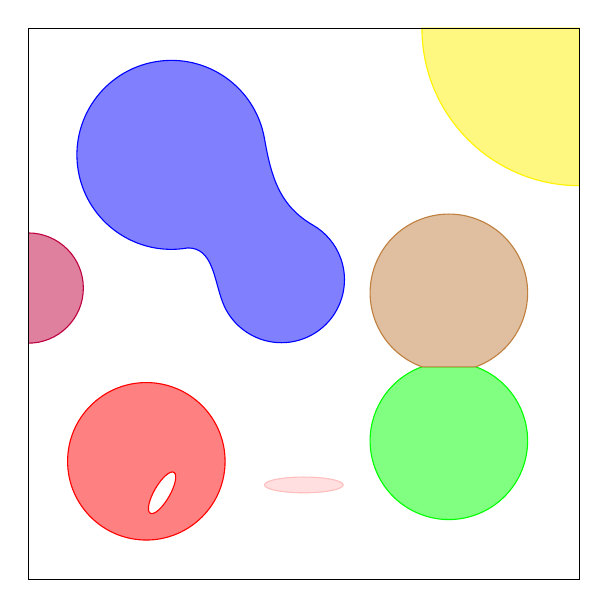
\begin{tikzpicture}[scale=1]
			\coordinate (porosity) at (1.7, 1.1);
			\draw[red, fill=red!50] (1.5,1.5) circle (1);
			\draw[red, fill=white, rotate=60] (porosity) ellipse (0.3 and 0.1);
			\draw[purple, fill=purple!50] (0,3) arc (-90:90:0.7);
			\draw[pink, fill=pink!50] (3.5,1.2) ellipse (0.5 and 0.1);
			\begin{scope}[shift={(3,5.6)}, rotate=-50]
				\draw[blue, fill=blue!50] (0,0) arc (60:360-30:1.2) to[out=50, in=160] ++(0.8,-0.1) arc (-110:110:0.8) to[out=200, in=-30] (0,0);
			\end{scope}
			\draw[yellow, fill=yellow!50] (5,7) arc (180:270:2) -- (7,7) -- cycle;
			\draw[green, fill=green!50] (5,2.7) arc (110:430:1) -- cycle;
			\draw[brown, fill=brown!50] (5,2.7) arc (250:-70:1) -- cycle;
			\draw (0,0) rectangle (7,7);
		\end{tikzpicture}
		}\hfill
		\subfloat[Image seuillée.]{
		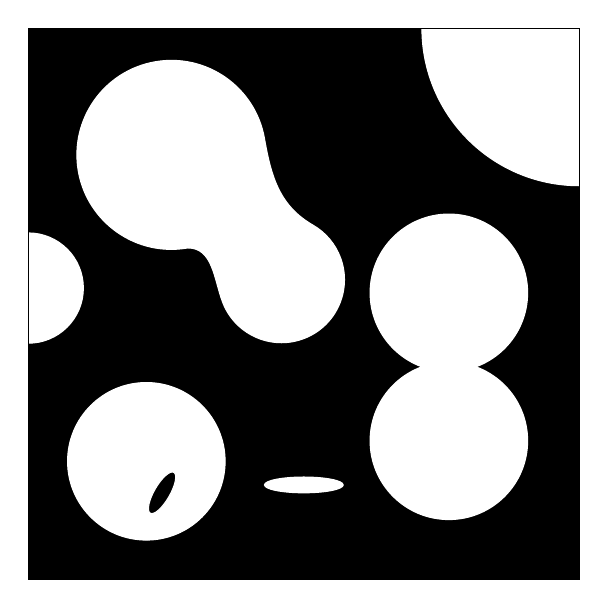
\begin{tikzpicture}[scale=1]
			\coordinate (porosity) at (1.7, 1.1);
			\fill[black] (0,0) rectangle (7,7);
			\draw[white, fill=white] (1.5,1.5) circle (1);
			\draw[white, fill=black, rotate=60] (porosity) ellipse (0.3 and 0.1);
			\draw[white, fill=white] (0,3) arc (-90:90:0.7);
			\draw[white, fill=white] (3.5,1.2) ellipse (0.5 and 0.1);
			\begin{scope}[shift={(3,5.6)}, rotate=-50]
				\draw[white, fill=white] (0,0) arc (60:360-30:1.2) to[out=50, in=160] ++(0.8,-0.1) arc (-110:110:0.8) to[out=200, in=-30] (0,0);
			\end{scope}
			\draw[white, fill=white] (5,7) arc (180:270:2) -- (7,7) -- cycle;
			\draw[white, fill=white] ({5-cos(110)},{2.7-sin(110)}) circle (1);
			\draw[white, fill=white] ({5-cos(110)},{2.7+sin(110)}) circle (1);
			\draw (0,0) rectangle (7,7);
		\end{tikzpicture}
		}
		\caption{\label{fig05:schema_segm}Schématisation d'un milieu granulaire observé par tomographie en vue d'expliquer le processus de segmentation. Une coupe du milieu granulaire réel est représenté en (a) tandis que (b) représente son image après seuillage.}
	\end{figure}
	\paragraph{(a) Pré-traitement de l'image binaire -}\label{para05:etapeA}
		\begin{figure}\centering
			\subfloat[Masque de la phase solide. Les traits en pointillés représentent la frontière de l'image seuillée.]{
			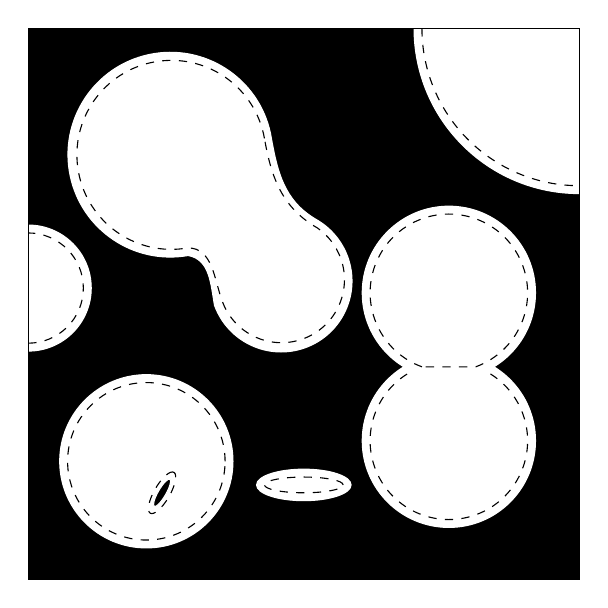
\begin{tikzpicture}[scale=1]
				\coordinate (porosity) at (1.7, 1.1);
				\fill[black] (0,0) rectangle (7,7);
				\draw[white, fill=white] (1.5,1.5) circle (1.1);
				\draw[dashed] (1.5,1.5) circle (1);
				\draw[dashed, rotate=60] (porosity) ellipse (0.3 and 0.1);
				\draw[white, fill=black, rotate=60] (porosity) ellipse (0.2 and 0.05);
				\draw[white, fill=white] (0,2.9) arc (-90:90:0.8);
				\draw[dashed] (0,3) arc (-90:90:0.7);
				\draw[white, fill=white] (3.5,1.2) ellipse (0.6 and 0.2);
				\draw[dashed] (3.5,1.2) ellipse (0.5 and 0.1);
				\begin{scope}[shift={(3,5.6)}, rotate=-50]
					\draw[white, fill=white] (0,0.1) arc (62:360-30:1.3) to[out=40, in=150] ++(0.7,-0.15) arc (-110:110:0.9) to[out=200, in=-30] (0,0.1);
					\draw[dashed] (0,0) arc (60:360-30:1.2) to[out=50, in=160] ++(0.8,-0.1) arc (-110:105:0.8) to[out=200, in=-30] (0,0);
				\end{scope}
				\draw[white, fill=white] (4.9,7) arc (180:270:2.1) -- (7,7) -- cycle;
				\draw[dashed] (5,7) arc (180:270:2);
				\draw[white, fill=white] ({5-cos(110)},{2.7-sin(110)}) circle (1.1);
				\draw[dashed] (5,2.7) arc (110:430:1);
				\draw[white, fill=white] ({5-cos(110)},{2.7+sin(110)}) circle (1.1);
				\draw[dashed] (5,2.7) arc (250:-70:1) -- cycle;
				\draw (0,0) rectangle (7,7);
			\end{tikzpicture}
			}\hfill
			\subfloat[Retrait des porosités dans le masque de la phase solide.]{
			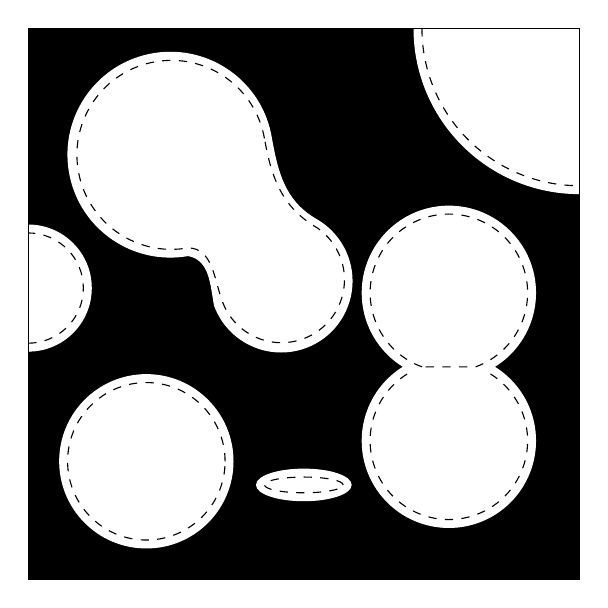
\begin{tikzpicture}[scale=1]
				\coordinate (porosity) at (1.7, 1.1);
				\fill[black] (0,0) rectangle (7,7);
				\draw[white, fill=white] (1.5,1.5) circle (1.1);
				\draw[dashed] (1.5,1.5) circle (1);
				\draw[white, fill=white] (0,2.9) arc (-90:90:0.8);
				\draw[dashed] (0,3) arc (-90:90:0.7);
				\draw[white, fill=white] (3.5,1.2) ellipse (0.6 and 0.2);
				\draw[dashed] (3.5,1.2) ellipse (0.5 and 0.1);
				\begin{scope}[shift={(3,5.6)}, rotate=-50]
					\draw[white, fill=white] (0,0.1) arc (62:360-30:1.3) to[out=40, in=150] ++(0.7,-0.15) arc (-110:110:0.9) to[out=200, in=-30] (0,0.1);
					\draw[dashed] (0,0) arc (60:360-30:1.2) to[out=50, in=160] ++(0.8,-0.1) arc (-110:105:0.8) to[out=200, in=-30] (0,0);
				\end{scope}
				\draw[white, fill=white] (4.9,7) arc (180:270:2.1) -- (7,7) -- cycle;
				\draw[dashed] (5,7) arc (180:270:2);
				\draw[white, fill=white] ({5-cos(110)},{2.7-sin(110)}) circle (1.1);
				\draw[dashed] (5,2.7) arc (110:430:1);
				\draw[white, fill=white] ({5-cos(110)},{2.7+sin(110)}) circle (1.1);
				\draw[dashed] (5,2.7) arc (250:-70:1) -- cycle;
				\draw (0,0) rectangle (7,7);
			\end{tikzpicture}
			}
			\caption{\label{fig05:imProc_preTraitement}Création du masque de la phase solide (a) et élimination des porosités internes (b) à partir de l'image seuillée.}
		\end{figure}
		La première étape consiste à utiliser l'image seuillée (figure \ref{fig05:schema_segm}-(b)) pour définir un masque\footnote{En traitement d'images, un masque correspond à une image binaire, de la même taille que l'image traitée, pour laquelle une zone de l'image traitée va prendre la valeur \num{1} tandis que la partie complémentaire prend la valeur \num{0}. De nombreuses fonctions prennent en argument un masque afin de traiter uniquement la zone positive.} 3D qui qualifie une zone de certitude concernant l'appartenance à la phase solide. En continuant de considérer les voxels dont la valeur vaut \num{1}  comme voxels appartenant à la phase solide (inversement \num{0} pour la phase gazeuse), une dilatation de l'image seuillée suffit à ajouter tous les voxels à la frontière entre les deux phases du côté des grains (figure \ref{fig05:imProc_preTraitement}-(a)). S'il existe des erreurs d'appartenance des voxels liées au seuillage, on diminue grandement cette erreur en procédant ainsi. Le masque obtenu par la dilatation 3D est appelé dans le suite "masque de la phase solide". Dans ce masque, les valeurs nulles représentent les zones inactives du masque ; les zones non nulles sont les zones actives du masque (les zones noires et blanches, respectivement, dans la figure \ref{fig05:imProc_preTraitement}-(a)). En plus de cela, pour des raisons qui vont être évoquées dans le prochain paragraphe, il est nécessaire de fermer toute potentielle porosité à l'intérieur des grains. Après correction des images, ces porosités sont très peu nombreuses mais peuvent bien être présentes. Une manière de faire cela est de soumettre à l'image plusieurs dilatations (au moins autant que le rayon moyen des porosités en taille de voxel) puis de soumettre le même nombre d'érosions (figure \ref{fig05:imProc_preTraitement}-(b)). Il s'agit ni plus ni moins d'une fermeture avec plusieurs itérations (cf. paragraphe \ref{para03:traitement_image}).
	\paragraph{(b) Définition des marqueurs associés aux grains -}
		L'objectif de cette étape est de définir le nombre de particules présentes dans l'image.
		\subparagraph{Méthode "idéale" :}En considérant un milieu monodisperse, dont les particules ont des géométries plutôt convexes et avec des zones de contact de petite taille, il paraît pertinent de définir le nombre de particules en sélectionnant le centre géométrique de chacune d'entre elles. Une manière simple de faire cela est de procéder au calcul d'une carte des distances en 3D et de seuiller l'image de manière à ne considérer que les zones centrales des grains. La carte des distances est calculée par l'intermédiaire d'une fonction qui calcule, pour chaque voxel de l'image issue de l'étape précédente et constituant la phase solide, la distance euclidienne qui le sépare du plus proche voxel constituant la phase non solide. En sortie, le voxel prend comme valeur cette distance. De cette manière, si aucune porosité interne n'est présente - d'où le post-traitement de la première étape - alors les voxels les plus éloignés de la frontière des grains (donc les zones centrales) ont une valeur plus élevée que la moyenne et il est possible de les isoler par une étape de seuillage. Dans ce cas, il est nécessaire de déterminer une valeur seuil définissant la limite des zones centrales, qui sont appelées "marqueurs".
		\subparagraph{Méthode "adaptée" :}
		\begin{figure}\centering
			\subfloat[Carte des distances du masque de la phase solide]{
			\begin{tikzpicture}[scale=1]
				\node (P) at (3.5,3.5)  {\includegraphics[width=7cm]{segmentation/illustration_EDT.png}};
			\end{tikzpicture}
			}\hfill
			\subfloat[Recherche des maxima locaux.]{
			\begin{tikzpicture}[scale=1]
				\node (P) at (3.5,3.5)  {\includegraphics[width=7cm]{segmentation/illustration_EDT.png}};
				\coordinate (G1) at (1.5,1.45);
				\coordinate (G2) at (0.1,3.65);
				\coordinate (G3) at (3.5,1.15);
				\coordinate (G4a) at (1.8,5.4);
				\coordinate (G4b) at (3.2,3.7);
				\coordinate (G5) at (6.8,6.8);
				\coordinate (G6) at ({5.15-cos(110)}, {2.65-sin(110)});
				\coordinate (G7) at ({5.15-cos(110)}, {2.65+sin(110)});
				% dessine les marqueurs
				\draw[red] (G1) node {$\bullet$};
				\draw[red] (G2) node {$\bullet$};
				\draw[red] (G3) node {$\bullet$};
				\draw[red] (G4a) node {$\bullet$};
				\draw[red] (G4b) node {$\bullet$};
				\draw[red] (G5) node {$\bullet$};
				\draw[red] (G6) node {$\bullet$};
				\draw[red] (G7) node {$\bullet$};
			\end{tikzpicture}
			}\\
			\subfloat[Marqueurs issus du seuillage de la carte des distances.]{
			\begin{tikzpicture}[scale=1]
				\draw (0,0) rectangle (7,7);
				\coordinate (G1) at (1.5,1.45);
				\coordinate (G2) at (0.1,3.65);
				\coordinate (G3) at (3.5,1.15);
				\coordinate (G4a) at (1.8,5.4);
				\coordinate (G4b) at (3.2,3.7);
				\coordinate (G5) at (6.8,6.8);
				\coordinate (G6) at ({5.15-cos(110)}, {2.65-sin(110)});
				\coordinate (G7) at ({5.15-cos(110)}, {2.65+sin(110)});
				% dessine les marqueurs
				\draw[red] (G1) node {$\bullet$};
				\draw[red] (G2) node {$\bullet$};
				\draw[red] (G3) node {$\bullet$};
				\draw[red] (G4a) node {$\bullet$};
				\draw[red] (G4b) node {$\bullet$};
				\draw[red] (G5) node {$\bullet$};
				\draw[red] (G6) node {$\bullet$};
				\draw[red] (G7) node {$\bullet$};
			\end{tikzpicture}
			}\hfill
			\subfloat[Labellisation des marqueurs.]{
			\begin{tikzpicture}[scale=1]
				\draw (0,0) rectangle (7,7);
				\coordinate (G1) at (1.5,1.45);
				\coordinate (G2) at (0.1,3.65);
				\coordinate (G3) at (3.5,1.15);
				\coordinate (G4a) at (1.8,5.4);
				\coordinate (G4b) at (3.2,3.7);
				\coordinate (G5) at (6.8,6.8);
				\coordinate (G6) at ({5.15-cos(110)}, {2.65-sin(110)});
				\coordinate (G7) at ({5.15-cos(110)}, {2.65+sin(110)});
				% dessine les marqueurs
				\draw[red] (G1) node {$\bullet$};
				\draw[purple] (G2) node {$\bullet$};
				\draw[pink] (G3) node {$\bullet$};
				\draw[blue] (G4a) node {$\bullet$};
				\draw[gray] (G4b) node {$\bullet$};
				\draw[yellow] (G5) node {$\bullet$};
				\draw[green] (G6) node {$\bullet$};
				\draw[brown] (G7) node {$\bullet$};
			\end{tikzpicture}
			}
			\caption{\label{fig05:imProc_markers}Identification des marqueurs à partir de la carte des distances du masque de la phase solide (a). Les maxima locaux sont recherchés (b) afin de créer une image de marqueurs (c). Chacun des marqueur est labellisé de manière à ce qu'il soit unique (d).}
		\end{figure}
		La méthode présentée ci-dessus est adaptée aux milieux granulaires présentant certaines caractéristiques : monodispersité, géométrie des grains régulière et convexe et zones de contact de petites tailles. Ces conditions permettent en effet de pouvoir s'assurer de l'existence d'une seule zone d'intensité élevée dans chaque grain, et dont l'intensité est sensiblement la même pour chacun d'entre eux. L'observation de la figure \ref{fig04:contrast_enhancement_filtering} rend compte du fait que les conditions précitées ne sont pas réunies pour les échantillons de polystyrène. Pour ces raisons, une stratégie a été établie : le calcul de la carte des distances à partir du masque de la phase solide reste inchangé (figure \ref{fig05:imProc_markers}-(a)) mais il est choisi de ne pas utiliser une méthode de seuillage pour reconnaître le nombre de grains mais de favoriser une méthode qui surestime ce nombre. En faisant cela, chaque grain réel sera reconnu comme un ensemble de plusieurs "grains numériques" qu'il sera ensuite possible de rassembler en un seul grain numérique. La méthode qui consiste à déterminer les différents marqueurs\footnote{Pour rappel, un marqueur correspond à une zone définie par une nuance de gris. Les marqueurs sont utilisés par la suite dans des fonctions qui ont besoin de reconnaître les différentes zones.} au sein des grains est basée sur une fonction du module Python de "scikit-image" \citep{scikit_image} qui recherche les maxima locaux dans les images 3D en faisant en sorte que ces derniers soient séparés l'un de l'autre d'une distance minimale déterminé par l'utilisateur (figure \ref{fig05:imProc_markers}-(b)). Les maxima locaux trouvés sont de la taille d'un voxel par défaut. Afin de créer des marqueurs suffisamment larges, quelques dilatations sont faites. Enfin, il faut que chacun des marqueurs (figure \ref{fig05:imProc_markers}-(c)) soit unique, c'est-à-dire qu'il lui est attribué un niveau de gris qui ne peut être commun avec aucun autre voxel de l'image. Pour cela, l'image contenant les marqueurs est labellisée : il s'agit d'un processus d'identification des zones isolées dans le volume et d'attribution de valeurs uniques pour chacune de ces zones (figure \ref{fig05:imProc_markers}-(d)). Avec la labellisation chaque marqueur sera identifié à un label, qui n'est autre que la nuance de gris utilisée pour identifier le marqueur. Si le nombre de marqueurs est supérieur à \num{255} ($2^8-1$) alors l'image des marqueurs doit être enregistrée au format 16-bit qui admet un nombre maximal de marqueur de \num{65535} ($2^{16}-1$). Les labels prennent des valeurs strictement supérieures à \num{0}. En effet, la valeur \num{0} est attribuée aux zones de porosité.
	\paragraph{(c) Premier watershed -}
		\begin{figure}
			\subfloat[Image de tomographie utilisée dans le watershed avec les marqueurs. La zone grisée est la zone inactive du masque de la phase solide et n'est pas traitée. les traits en pointillés indiquent les frontières réelles.]{
			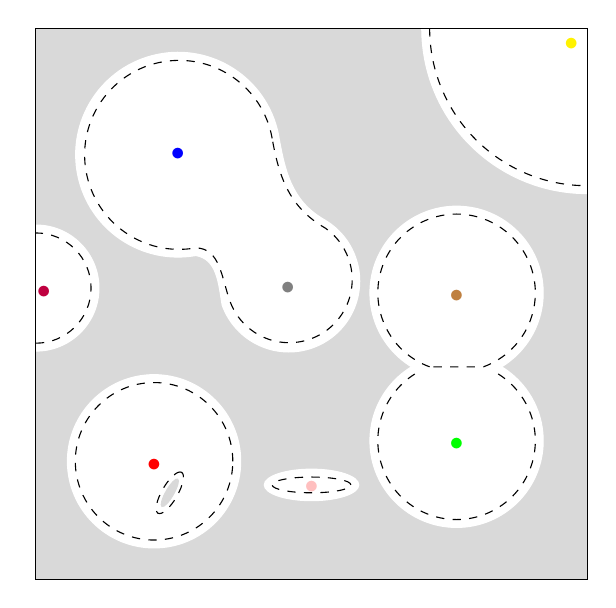
\begin{tikzpicture}[scale=1.]
				\coordinate (G1) at (1.5,1.45);
				\coordinate (G2) at (0.1,3.65);
				\coordinate (G3) at (3.5,1.17);
				\coordinate (G4a) at (1.8,5.4);
				\coordinate (G4b) at (3.2,3.7);
				\coordinate (G5) at (6.8,6.8);
				\coordinate (G6) at ({5-cos(110)}, {2.65-sin(110)});
				\coordinate (G7) at ({5-cos(110)}, {2.65+sin(110)});
				\coordinate (porosity) at (1.7, 1.1);
				\fill[gray!30] (0,0) rectangle (7,7);
				\draw[white, fill=white] (1.5,1.5) circle (1.1);
				\draw[dashed] (1.5,1.5) circle (1);
				\draw[white, fill=white] (0,2.9) arc (-90:90:0.8);
				\draw[dashed] (0,3) arc (-90:90:0.7);
				\draw[dashed, rotate=60] (porosity) ellipse (0.3 and 0.1);
				\draw[gray!30, fill=gray!30, rotate=60] (porosity) ellipse (0.2 and 0.05);
				\draw[white, fill=white] (3.5,1.2) ellipse (0.6 and 0.2);
				\draw[dashed] (3.5,1.2) ellipse (0.5 and 0.1);
				\begin{scope}[shift={(3,5.6)}, rotate=-50]
					\draw[white, fill=white] (0,0.1) arc (62:360-30:1.3) to[out=40, in=150] ++(0.7,-0.15) arc (-110:110:0.9) to[out=200, in=-30] (0,0.1);
					\draw[dashed] (0,0) arc (60:360-30:1.2) to[out=50, in=160] ++(0.8,-0.1) arc (-110:105:0.8) to[out=200, in=-30] (0,0);
				\end{scope}
				\draw[white, fill=white] (4.9,7) arc (180:270:2.1) -- (7,7) -- cycle;
				\draw[dashed] (5,7) arc (180:270:2);
				\draw[white, fill=white] ({5-cos(110)},{2.7-sin(110)}) circle (1.1);
				\draw[dashed] (5,2.7) arc (110:430:1);
				\draw[white, fill=white] ({5-cos(110)},{2.7+sin(110)}) circle (1.1);
				\draw[dashed] (5,2.7) arc (250:-70:1) -- cycle;
				\draw[] (0,0) rectangle (7,7);
				% dessine les marqueurs
				\draw[red] (G1) node {$\bullet$};
				\draw[purple] (G2) node {$\bullet$};
				\draw[pink] (G3) node {$\bullet$};
				\draw[blue] (G4a) node {$\bullet$};
				\draw[gray] (G4b) node {$\bullet$};
				\draw[yellow] (G5) node {$\bullet$};
				\draw[green] (G6) node {$\bullet$};
				\draw[brown] (G7) node {$\bullet$};
			\end{tikzpicture}
			}\hfill
			\subfloat[Résultat de la première propagation des marqueurs par la fonction watershed. Les traits en pointillés sont les frontières réelles tandis que les zones colorées sont les labels. Une érosion est réalisée à la fin du watershed.]{
			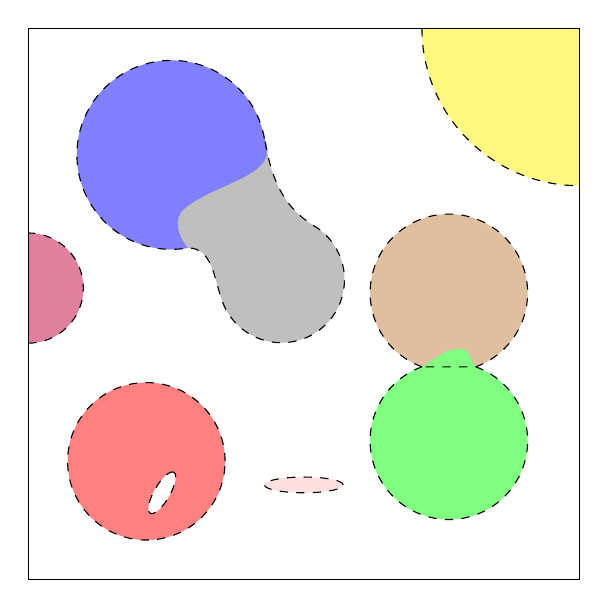
\begin{tikzpicture}[scale=1.]
				\coordinate (porosity) at (1.7, 1.1);
				\draw[dashed, fill=red!50] (1.5,1.5) circle (1);
				\draw[dashed, fill=white, rotate=60] (porosity) ellipse (0.3 and 0.1);
				\draw[dashed, fill=purple!50] (0,3) arc (-90:90:0.7);
				\draw[dashed, fill=pink!50] (3.5,1.2) ellipse (0.5 and 0.1);
				\begin{scope}[shift={(3,5.6)}, rotate=-50]
					\fill[gray!50] (0,0) arc (60:360-30:1.2) to[out=50, in=160] ++(0.8,-0.1) arc (-110:105:0.8) to[out=200, in=-30] (0,0);
					\fill[blue!50] (0,0) arc (60:360-30:1.2) to[out=180, in=180+90] ++(180-35:0.5) to[out=90, in=-15] cycle;
					\draw[dashed] (0,0) arc (60:360-30:1.2) to[out=50, in=160] ++(0.8,-0.1) arc (-110:105:0.8) to[out=200, in=-30] (0,0);
				\end{scope}
				\fill[yellow!50] (5,7) arc (180:270:2) -- (7,7) -- cycle;
				\draw[dashed] (5,7) arc (180:270:2);
				\fill[green!50] (5,2.7) arc (110:430:1) to[out=90, in=0] ++(125:0.4) to[out=180, in=90] cycle;
				\fill[brown!50] (5,2.7) arc (250:-70:1) to[out=130, in=0] ++(130:0.3) to[out=180, in=30] cycle;
				\draw[dashed] (5,2.7) arc (110:430:1);
				\draw[dashed] (5,2.7) arc (250:-70:1) -- cycle;
				\draw[] (0,0) rectangle (7,7);
			\end{tikzpicture}
			}
			\caption{\label{fig05:imProc_WS1}Watershed réalisé à partir des marqueurs labellisés et basé sur le contraste de l'image de tomographie.}
		\end{figure}
		Le lecteur peut se ramener au paragraphe \ref{para03:traitement_image} pour comprendre l'action de la fonction watershed. Cette fonction nécessite trois images en entrée et crée une image en sortie. Les images d'entrée sont :
		\begin{itemize}
			\item L'image contenant les différents marqueurs, correspondant aux différents lacs.
			\item L'image originale (post-traitée) en niveaux de gris dans laquelle les marqueurs vont se propager, cela correspond à la montée des eaux à partir des lacs.
			\item Le masque de la phase solide qui permet de travailler uniquement dans la zone de présence certaine des grains. L'objectif est ici de diminuer la puissance de calcul nécessaire pour traiter l'image entière. Les zones inactives du masque correspondent à des digues : la montée des eaux ne concerne pas ces zones.
		\end{itemize}
		La figure \ref{fig05:imProc_WS1}-(a) est une schématisation de ce que la fonction watershed prend en entrée. L'image de sortie représente le volume dans lequel les zones inactives du masque de la phase solide sont des porosités (marqueur de valeur \num{0}) et les zones actives sont comblées par des zones labellisées issues de la propagation des marqueurs. Les zones labellisées seront appelées dans la suite "labels". Puisque plusieurs marqueurs sont potentiellement présents dans un même grain initialement, l'intégralité de ce même grain sera constitué du même nombre de labels que de marqueurs à la fin du watershed (figure \ref{fig05:imProc_WS1}-(b)).
		
	\paragraph{(d) Analyse et correction des contacts -}
		\begin{figure}\centering
			\subfloat[Mesure de la surface totale des labels (surfaces de la même couleur que les labels + surfaces oranges pour les labels qui ont un contact) et des surfaces de contact (en orange).]{
			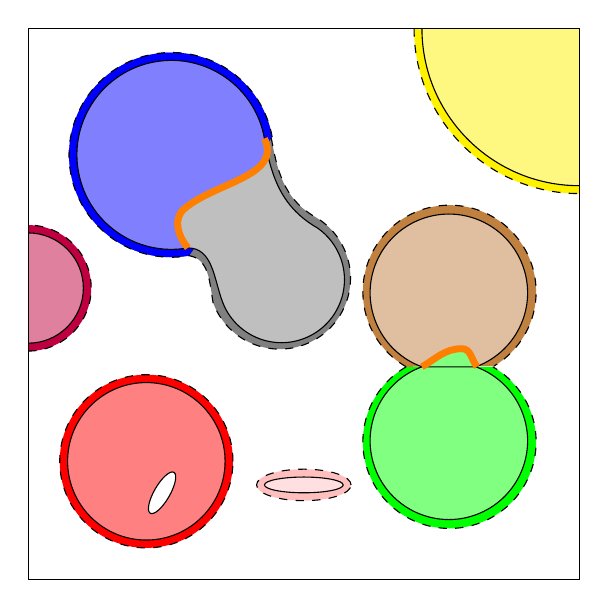
\begin{tikzpicture}[scale=1.]
			\coordinate (porosity) at (1.7, 1.1);
			\draw[dashed, fill=red] (1.5,1.5) circle (1.1);
			\draw[fill=red!50] (1.5,1.5) circle (1);
			\draw[fill=white, rotate=60] (porosity) ellipse (0.3 and 0.1);
			\draw[dashed, fill=purple] (0,2.9) arc (-90:90:0.8);
			\draw[fill=purple!50] (0,3) arc (-90:90:0.7);
			\draw[dashed, fill=pink] (3.5,1.2) ellipse (0.6 and 0.2);
			\draw[fill=pink!50] (3.5,1.2) ellipse (0.5 and 0.1);
			\begin{scope}[shift={(3,5.6)}, rotate=-50]
				\fill[gray] ({0.1*cos(60)},{0.1*sin(60)}) arc (60:360-30:1.3) to[out=40, in=150] ++(0.65,-0.15) arc (-110:110:0.9) to[out=200, in=-30] (0,0.1);
				\fill[blue] ({0.1*cos(60)},{0.1*sin(60)}) arc (60:360-30:1.3) -- cycle;
				\fill[gray!50] (0,0) arc (60:360-30:1.2) to[out=50, in=160] ++(0.8,-0.1) arc (-110:105:0.8) to[out=200, in=-30] (0,0);
				\fill[blue!50] (0,0) arc (60:360-30:1.2) to[out=180, in=180+90] ++(180-35:0.5) to[out=90, in=-15] cycle;
				\draw[] (0,0) arc (60:360-30:1.2) to[out=50, in=160] ++(0.8,-0.1) arc (-110:105:0.8) to[out=200, in=-30] (0,0);
				\draw[dashed] ({0.1*cos(60)},{0.1*sin(60)}) arc (60:360-30:1.3) to[out=40, in=150] ++(0.65,-0.15) arc (-110:110:0.9) to[out=200, in=-30] (0,0.1);
				\draw[orange, line width=0.25em] (240:1.2) ++(360-30:1.2) to[out=180, in=180+90] ++(180-35:0.5) to[out=90, in=-15] (0,0);
			\end{scope}
			\fill[yellow] (4.9,7) arc (180:270:2.1) -- (7,7) -- cycle;
			\fill[yellow!50] (5,7) arc (180:270:2) -- (7,7) -- cycle;
			\draw[dashed] (4.9,7) arc (180:270:2.1);
			\draw[] (5,7) arc (180:270:2);
			\draw[dashed, fill=green] (4.8,2.7) arc (120:420:1.1);
			\draw[dashed, fill=brown] (4.8,2.7) arc (240:-59:1.1);
			\fill[green!50] (5,2.7) arc (110:430:1) to[out=90, in=0] ++(125:0.4) to[out=180, in=90] cycle;
			\fill[brown!50] (5,2.7) arc (250:-70:1) to[out=130, in=0] ++(130:0.3) to[out=180, in=30] cycle;
			\draw[] (5,2.7) arc (110:430:1);
			\draw[] (5,2.7) arc (250:-70:1) -- cycle;
			\draw[orange, line width=0.25em] (5.7,2.7) to[out=130, in=0] ++(130:0.3) to[out=180, in=30] (5,2.7);
			\draw[] (0,0) rectangle (7,7);
			\end{tikzpicture}
			}\hfill
			\subfloat[Correction des contacts. Les contacts dont la surface est petite par rapport à la surface des labels sont conservés. Les autres sont retirés.]{
			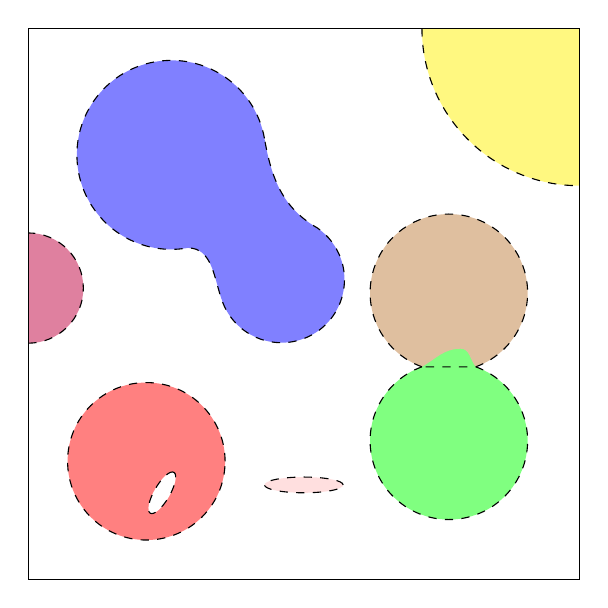
\begin{tikzpicture}[scale=1.]
				\coordinate (porosity) at (1.7, 1.1);
				\draw[dashed, fill=red!50] (1.5,1.5) circle (1);
				\draw[dashed, fill=white, rotate=60] (porosity) ellipse (0.3 and 0.1);
				\draw[dashed, fill=purple!50] (0,3) arc (-90:90:0.7);
				\draw[dashed, fill=pink!50] (3.5,1.2) ellipse (0.5 and 0.1);
				\begin{scope}[shift={(3,5.6)}, rotate=-50]
					\fill[blue!50] (0,0) arc (60:360-30:1.2) to[out=50, in=160] ++(0.8,-0.1) arc (-110:105:0.8) to[out=200, in=-30] (0,0);
					\draw[dashed] (0,0) arc (60:360-30:1.2) to[out=50, in=160] ++(0.8,-0.1) arc (-110:105:0.8) to[out=200, in=-30] (0,0);
				\end{scope}
				\fill[yellow!50] (5,7) arc (180:270:2) -- (7,7) -- cycle;
				\draw[dashed] (5,7) arc (180:270:2);
				\fill[green!50] (5,2.7) arc (110:430:1) to[out=90, in=0] ++(125:0.4) to[out=180, in=90] cycle;
				\fill[brown!50] (5,2.7) arc (250:-70:1) to[out=130, in=0] ++(130:0.3) to[out=180, in=30] cycle;
				\draw[dashed] (5,2.7) arc (110:430:1);
				\draw[dashed] (5,2.7) arc (250:-70:1) -- cycle;
				\draw[] (0,0) rectangle (7,7);
			\end{tikzpicture}
			}
			\caption{\label{fig05:imProc_contacts}Méthode d'analyse et de correction des contacts}
		\end{figure}
		\`A l'issue de l'étape précédente, les grains sont identifiés comme un assemblage de labels. L'objectif de cette étape est d'analyser les zones de contact entre labels (zones oranges sur la figure \ref{fig05:imProc_contacts}-(a)) et reconnaître les contacts réels des grains par rapport aux contacts qui n'en sont pas dans l'échantillon. Le voisinage de chacun des labels est étudié afin d'établir une première liste des contacts et d'analyser les surfaces totales et en contact pour chacun des labels. L'analyse de chacune des paires de labels en contact est ensuite effectuée afin de vérifier la condition donnée par l'équation (\ref{eq05:contacts}) :
		\begin{equation}\label{eq05:contacts}
			\textrm{Si}\qquad \cfrac{S_{(i,j)}}{\min{(S_i, S_j)}}>S_C \qquad\textrm{alors}\qquad i=j \qquad\textrm{sinon}\qquad  i\neq j
		\end{equation}
		où, $S_{(i,j)}$ est la surface de contact entre les labels numérotés $i$ et $j$, $S_i$ et $S_j$ sont respectivement les surfaces totales des labels numérotés $i$ et $j$ et $S_C$ est une valeur seuil comprise entre \num{0} et \num{1} déterminée par l'utilisateur. Si toutes les valeurs sont données en voxel, $S_{(i,j)}$ correspond au nombre de voxels du label $i$ qui touchent les voxels du label $j$ (ou l'inverse), la surface totale $S_i$ correspond au nombre de voxels entourant le label $i$ (en comptant également les zones de contact). Les surfaces $S_i$ sont obtenues en calculant le nombre de voxels de la structure engendrée par la différence du label dilaté (volume délimité par les traits en pointillés sur la figure \ref{fig05:imProc_contacts}-(a)) par le label lui-même (volume délimité par le trait plein sur la figure \ref{fig05:imProc_contacts}-(a)).
		\\Sachant cela, l'utilisateur doit choisir $S_C$ comme étant le ratio entre la plus grande surface de contact possible et la surface totale du plus petit label. $S_C$ est forcément compris entre $0$ et $1$. Posons $S_C=0.2$, pour chaque paire de labels en contact, si la zone de contact est supérieure à $20\%$ de la surface totale du plus petit label alors il il est considéré qu'il ne s'agit pas d'un contact réel et les deux labels sont rassemblés en un seul et même label. Au contraire, si le ratio des deux surfaces est inférieur alors il est considéré que les labels sont en contact l'un et l'autre. Sur l'exemple de la figure \ref{fig05:imProc_contacts}-(a), le ratio de la surface orange entre les labels verts et marrons et la surface du grain marron (le plus petit) est plus petit que le ratio choisi par l'utilisateur. Le résultat présenté sur la figure \ref{fig05:imProc_contacts}-(b) montre que les deux labels sont conservés. La seconde surface orange sur la même figure montre le cas où le ratio est plus grand que la valeur seuil : les deux labels (bleu et gris) sont rassemblés en un seul (bleu). Après cette analyse, l'image issue de l'étape précédente est directement corrigée afin de déterminer les nouvelles valeurs des labels. Sur cette nouvelle image, les labels sont logiquement moins nombreux et plus volumineux en moyenne. Dans les travaux présentés ici, sur les reconstructions de tomographie du milieu constitué de polystyrène, la valeur de $S_c$  est de \num{0.15}.
		\\Il est supposé que le paramètre $S_C$ joue un rôle pouvant être non significatif sur les résultats de simulation. En effet, le choix d'un coefficient adapté permet une bonne définition des contacts entre grains et du nombre de grain total dans le volume simulé. Ainsi, les interactions de contact entre grains sont proches des interactions réelles et les conditions initiales sont établies de manière cohérente.
	\paragraph{(e) Correction de la frontière des grains par un second watershed -}
		\begin{figure}
			\subfloat[\'Erosions de chaque label pour former de nouveaux marqueurs.]{
			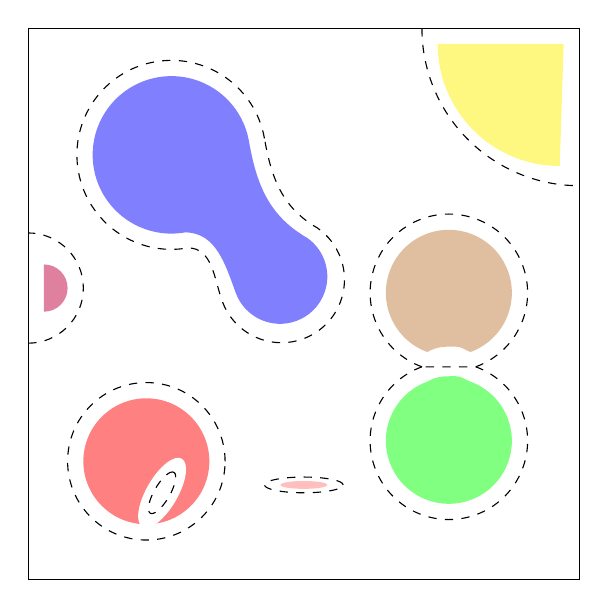
\begin{tikzpicture}[scale=1.]
				\coordinate (porosity) at (1.7, 1.1);
				\fill[red!50] (1.5,1.5) circle (0.8);
				\draw[dashed] (1.5,1.5) circle (1);
				\fill[white, rotate=60] (porosity) ellipse (0.5 and 0.2);
				\draw[dashed, rotate=60] (porosity) ellipse (0.3 and 0.1);
				\fill[purple!50] (0.2,3.4) arc (-90:90:0.3);
				\draw[dashed] (0,3) arc (-90:90:0.7);
				\fill[pink] (3.5,1.2) ellipse (0.3 and 0.05);
				\draw[dashed] (3.5,1.2) ellipse (0.5 and 0.1);
				\begin{scope}[shift={(3,5.6)}, rotate=-50]
					\draw[dashed] (0,0) arc (60:360-30:1.2) to[out=50, in=160] ++(0.8,-0.1) arc (-110:105:0.8) to[out=200, in=-30] (0,0);
					\fill[blue!50] (240:1.2) ++(60:1) arc (60:360-30:1.0) to[out=50, in=160] ++(1,0) arc (-110:105:0.6) to[out=200, in=-30] cycle;
				\end{scope}
				\fill[yellow!50] (5.2,6.8) arc (180:270:1.55) -- (6.8,6.8) -- cycle;
				\draw[dashed] (5,7) arc (180:270:2);
				\fill[green!50] ({5-cos(110)},{2.7-sin(110)}) ++(110:0.8) arc (110:430:0.8) to[out=160, in=0] ++(160:0.2) to[out=180, in=30] cycle;
				\fill[brown!50] ({5-cos(110)},{2.7+sin(110)}) ++(250:0.8) arc (250:-70:0.8) to[out=160, in=0] ++(160:0.2) to[out=180, in=30] cycle;
				\draw[dashed] (5,2.7) arc (110:430:1);
				\draw[dashed] (5,2.7) arc (250:-70:1) -- cycle;
				\draw[] (0,0) rectangle (7,7);
			\end{tikzpicture}
			}\hfill
			\subfloat[Second watershed avec propagation des nouveaux marqueurs compte tenu du contraste de l'image de tomographie.]{
			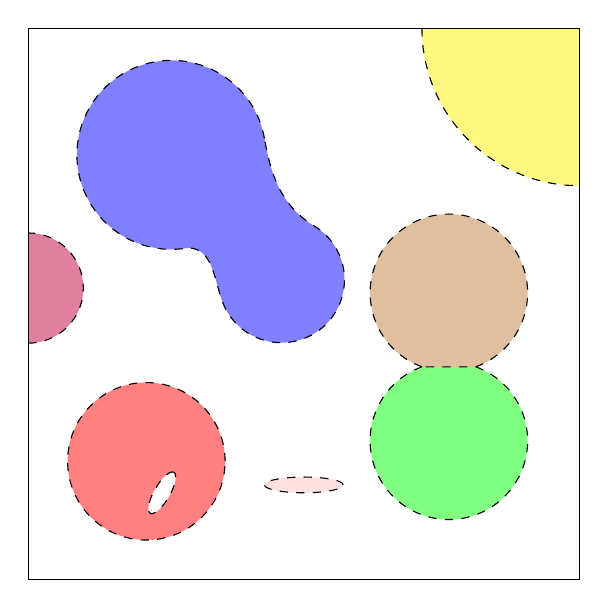
\begin{tikzpicture}[scale=1.]
				\coordinate (porosity) at (1.7, 1.1);
				\draw[dashed, fill=red!50] (1.5,1.5) circle (1);
				\draw[dashed, fill=white, rotate=60] (porosity) ellipse (0.3 and 0.1);
				\draw[dashed, fill=purple!50] (0,3) arc (-90:90:0.7);
				\draw[dashed, fill=pink!50] (3.5,1.2) ellipse (0.5 and 0.1);
				\begin{scope}[shift={(3,5.6)}, rotate=-50]
					\fill[blue!50] (0,0) arc (60:360-30:1.2) to[out=50, in=160] ++(0.8,-0.1) arc (-110:105:0.8) to[out=200, in=-30] (0,0);
					\draw[dashed] (0,0) arc (60:360-30:1.2) to[out=50, in=160] ++(0.8,-0.1) arc (-110:105:0.8) to[out=200, in=-30] (0,0);
				\end{scope}
				\fill[yellow!50] (5,7) arc (180:270:2) -- (7,7) -- cycle;
				\draw[dashed] (5,7) arc (180:270:2);
				\fill[green!50] (5,2.7) arc (110:430:1) -- cycle;
				\fill[brown!50] (5,2.7) arc (250:-70:1) -- cycle;
				\draw[dashed] (5,2.7) arc (110:430:1);
				\draw[dashed] (5,2.7) arc (250:-70:1) -- cycle;
				\draw[] (0,0) rectangle (7,7);
			\end{tikzpicture}
			}
			\caption{\label{fig05:imProc_frontiere} Correction de la frontière des grains par un second watershed.}
		\end{figure}
		Les étapes précédentes ont permis de déterminer, dans la limite du possible, un marqueur par particule et donc de déterminer le nombre de grains dans l'image à segmenter. Il reste désormais à trouver les frontières réelles entre les grains. Le problème de localisation de la frontière se retrouve dans les zones de contact entre labels. L'image issue de l'étape précédente présente un ensemble de labels qui, visuellement, semblent se superposer assez bien avec les grains observés en tomographie mais dont les zones de contact peuvent être erronées de quelques voxels. Il est donc nécessaire de résoudre ce problème en retirant les voxels les plus proches des frontières et en utilisant les labels ainsi obtenus comme nouveaux marqueurs qui vont se propager lors d'un second appel à l'algorithme de watershed. Quelques érosions itératives sont donc réalisées afin que les nouveaux marqueurs constituent la quasi-totalité des grains mais de telle sorte que la frontière des nouveaux marqueurs soit incluse à l'intérieur des grains observés sur les images de tomographie (figure \ref{fig05:imProc_frontiere}-(a)). Les nouveaux marqueurs sont ensuite utilisés dans la fonction watershed et une nouvelle propagation des labels, basée sur le contraste de l'image originale, est générée. Dans les zones éloignées des zones de contact, les nouveaux labels coïncident avec les anciens. Au niveau des zones de contact la frontière entre les grains est mieux établie puisque le contraste de l'image de tomographie associé à la faible distance entre les labels permet généralement de localiser correctement cette frontière (figure \ref{fig05:imProc_frontiere}-(b)).
	\paragraph{(f) Corrections de la géométrie 3D des grains -}
		\begin{figure}\centering
			\subfloat[Lissage de surface et élimination des porosités internes par des étapes de fermeture et ouverture successives.]{
			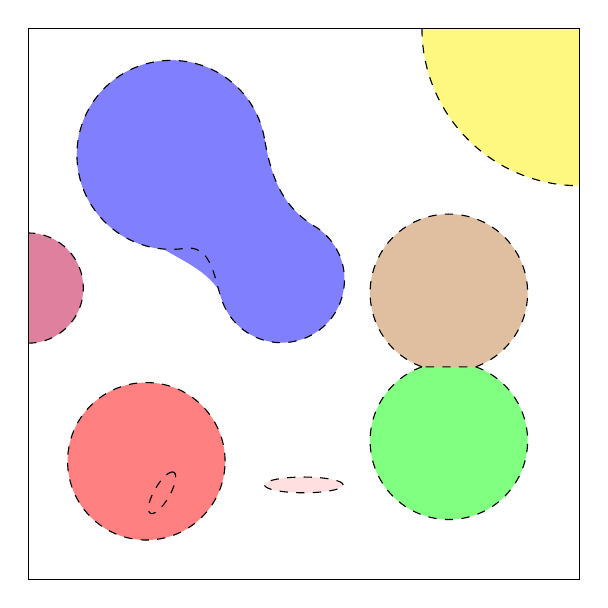
\begin{tikzpicture}[scale=1.]
				\coordinate (porosity) at (1.7, 1.1);
				\draw[dashed, fill=red!50] (1.5,1.5) circle (1);
				\draw[dashed, rotate=60] (porosity) ellipse (0.3 and 0.1);
				\draw[dashed, fill=purple!50] (0,3) arc (-90:90:0.7);
				\draw[dashed, fill=pink!50] (3.5,1.2) ellipse (0.5 and 0.1);
				\begin{scope}[shift={(3,5.6)}, rotate=-50]
					\fill[blue!50] (0,0) arc (60:360-30:1.2) to[out=50, in=160] ++(0.8,-0.1) arc (-110:105:0.8) to[out=200, in=-30] (0,0);
					\fill[blue!50] (0,0) arc (60:360-45:1.2) to[out=20, in=160] ++(1.1,0.15) -- cycle;
					\draw[dashed] (0,0) arc (60:360-30:1.2) to[out=50, in=160] ++(0.8,-0.1) arc (-110:105:0.8) to[out=200, in=-30] (0,0);
				\end{scope}
				\fill[yellow!50] (5,7) arc (180:270:2) -- (7,7) -- cycle;
				\draw[dashed] (5,7) arc (180:270:2);
				\fill[green!50] (5,2.7) arc (110:430:1) -- cycle;
				\fill[brown!50] (5,2.7) arc (250:-70:1) -- cycle;
				\draw[dashed] (5,2.7) arc (110:430:1);
				\draw[dashed] (5,2.7) arc (250:-70:1) -- cycle;
				\draw[] (0,0) rectangle (7,7);
			\end{tikzpicture}
			}\hfill
			\subfloat[Post-traitement : les labels trop petits sont retirés, les autres sont enregistrés.]{
			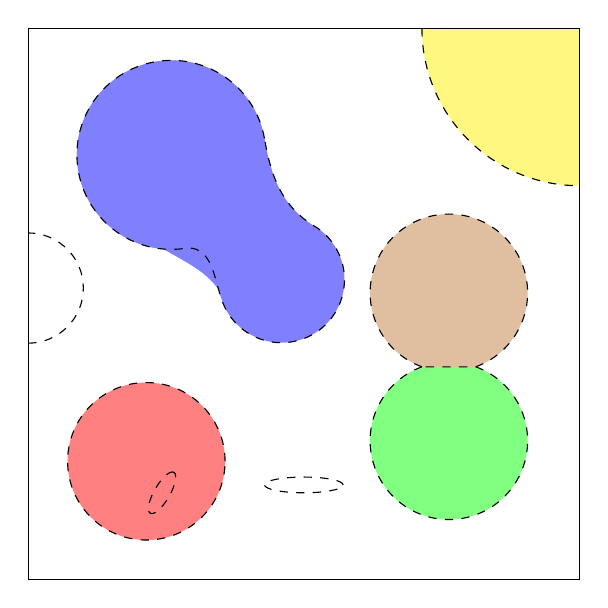
\begin{tikzpicture}[scale=1.]
				\coordinate (porosity) at (1.7, 1.1);
				\draw[dashed, fill=red!50] (1.5,1.5) circle (1);
				\draw[dashed, rotate=60] (porosity) ellipse (0.3 and 0.1);
				\draw[dashed] (0,3) arc (-90:90:0.7);
				\draw[dashed] (3.5,1.2) ellipse (0.5 and 0.1);
				\begin{scope}[shift={(3,5.6)}, rotate=-50]
					\fill[blue!50] (0,0) arc (60:360-30:1.2) to[out=50, in=160] ++(0.8,-0.1) arc (-110:105:0.8) to[out=200, in=-30] (0,0);
					\fill[blue!50] (0,0) arc (60:360-45:1.2) to[out=20, in=160] ++(1.1,0.15) -- cycle;
					\draw[dashed] (0,0) arc (60:360-30:1.2) to[out=50, in=160] ++(0.8,-0.1) arc (-110:105:0.8) to[out=200, in=-30] (0,0);
				\end{scope}
				\fill[yellow!50] (5,7) arc (180:270:2) -- (7,7) -- cycle;
				\draw[dashed] (5,7) arc (180:270:2);
				\fill[green!50] (5,2.7) arc (110:430:1) -- cycle;
				\fill[brown!50] (5,2.7) arc (250:-70:1) -- cycle;
				\draw[dashed] (5,2.7) arc (110:430:1);
				\draw[dashed] (5,2.7) arc (250:-70:1) -- cycle;
				\draw[] (0,0) rectangle (7,7);
			\end{tikzpicture}
			}
			\caption{\label{fig05:imProc_poro}Analyse et dernières modifications de l'image segmentée.}
		\end{figure}
		Une fois que les labels correspondent aux grains, une procédure itérative sur chaque label est réalisée de manière à lisser la surface des labels et éliminer les potentielles porosités (voxels dont la valeur d'intensité est \num{0}). Pour se faire, la succession d'une ouverture et d'une fermeture est réalisée (figure \ref{fig05:imProc_poro}-(a)). Cette étape est essentielle pour la suite puisqu'elle facilite le maillage (qui est présenté dans la partie \ref{para05:maillage}) et permet de définir des grains sans porosité interne.
	\paragraph{(g) Post-traitement de l'image segmentée -}\label{para05:post_segm}
		A l'issue de l'étape précédente chacune des particules constituant le milieu granulaire numérisé est enregistrée sous forme d'une image 3D. Cependant, certains grains sont trop petits pour être traités par la suite (maillage) et peuvent être, non des grains réels mais des artefacts liés au bruit résiduel dans l'image. Pour résoudre ce problème, il est nécessaire d'analyser le volume de chaque label et de vérifier qu'il est supérieur à une valeur limite de quelques voxels. Si tel n'est pas le cas, le label est supprimé (figure \ref{fig05:imProc_poro}-(b)).
		\\Une dernière étape consiste à préparer les phases de maillage et de simulation. Pour chacun des grains, un dossier est créé dans lequel est sauvegardé l'image 3D du label (le grain numérisé donc) ainsi qu'un fichier d'informations contenant un nom unique qui sera donné au grain, la position du grain\footnote{Il s'agit de la position d'un des sommets du parallélépipède qui englobe tout le grain. C'est ce sommet qui servira d'origine locale pour définir les coordonnées des n\oe{}uds dans la phase de maillage.} dans l'image 3D et dans l'image de tomographie ainsi que son volume en voxels.
	\paragraph{}
		\begin{figure}\centering
			~\hfill
			\subfloat[Image d'origine traitée]{\includegraphics[width=.3\textwidth]{segmentation/00_img_bilat_tv_crop_0099.jpg}}
			\hfill
			\subfloat[Image seuillée]{\includegraphics[width=.3\textwidth]{segmentation/01_img_filled_0114.jpg}}\hfill~\\
			\subfloat[Carte des distances]{\includegraphics[width=.3\textwidth]{segmentation/02_edt_0114.jpg}}\hfill
			\subfloat[Marqueurs (maxima locaux)]{\includegraphics[width=.3\textwidth]{segmentation/03_local_maxi_lab_0114.jpg}}\hfill
			\subfloat[Premier watershed]{\includegraphics[width=.3\textwidth]{segmentation/04_ws_loc_0114.jpg}}\\
			\subfloat[Correction des contacts]{\includegraphics[width=.3\textwidth]{segmentation/05_contacts.jpg}}\hfill
			\subfloat[Correction des frontières]{\includegraphics[width=.3\textwidth]{segmentation/06_labelled_tmp2_0114.jpg}}\hfill
			\subfloat[Correction de la géométrie et post-traitement]{\includegraphics[width=.3\textwidth]{segmentation/07_labelled_random_0099.jpg}}
			\caption{\label{fig05:process_segmentation}Visualisation du process de segmentation des grains de polystyrène sur une coupe 2D de la reconstruction de tomographie.}
		\end{figure}
		Il est possible d'observer l'effet de certaines de ces étapes sur la figure \ref{fig05:process_segmentation}. On remarque que la géométrie des grains n'est plus un frein à la segmentation des particules grâce à l'étape de correction des contacts après le premier watershed. L'image finale peut s'avérer quelque peu différente de l'image segmentée idéale puisque les filtres d'ouverture et fermeture en fin de processus modifient légèrement les bords des grains. La figure \ref{fig05:segmentation3D} permet de mieux visualiser le résultat de la segmentation sur des coupes 2D ainsi que sur une partie du volume.
		\begin{figure}\centering
			\subfloat[Coupe en $z=200$]{\begin{tikzpicture}
				\node (im1) at (0,0) {\includegraphics[width=4.5cm]{segmentation/200_orig.jpg}};
				\node (im2) at (5,0) {\includegraphics[width=4.5cm]{segmentation/200_label.jpg}};
				\node (im3) at (10,0) {\includegraphics[width=4.5cm]{segmentation/200_superpose.jpg}};
				\draw[text width=4.5cm, text centered] (0,-2.5) node[below] {Image d'origine traitée};
				\draw[text width=4.5cm, text centered] (5,-2.5) node[below] {Image segmentée};
				\draw[text width=4.5cm, text centered] (10,-2.5) node[below] {Superposition};
				\end{tikzpicture}}\\
			\subfloat[Vue 3D d'une partie des grains numérisés et d'une partie de l'image d'origine]{\includegraphics[width=0.7\textwidth]{segmentation/segmentation_3D.png}}
			\caption{\label{fig05:segmentation3D}Résultat de la segmentation sur deux coupes 2D et une partie du volume 3D (des défauts de couleur en périphérie des grains liés à une compression au format jpeg sont observables)}
		\end{figure}
	\paragraph{}
		Le lecteur qui souhaite connaître les capacités de l'algorithme de segmentation peut se référer à l'annexe \ref{annexe:capacites_segm}. Cette annexe présente de manière qualitative et quantitative l'efficacité et la robustesse de l'algorithme à segmenter des volumes dont le bruit et le flou sont relativement élevés. L'efficacité de l'algorithme à segmenter des volumes constitués de particules dont la géométrie est complexe a été démontrée dans les paragraphes précédents.

\section{Maillage des grains numérisés}\label{para05:maillage}
	\paragraph{}
	Avec les précisions données dans la partie \ref{para:methodes_simu}, la méthode des éléments finis multi-particules (MP-FEM) est adoptée pour assurer la modélisation du comportement mécanique des empilements granulaires soumis à de grandes déformations. Cette méthode a pour particularité de considérer chaque grain comme des solides maillés en volume auxquels il est possible d’associer des lois de comportement variées en fonction du matériau constitutif des grains. Il est courant pour cette méthode de mailler chaque grain avec un nombre d’éléments finis compris entre \num{300} et \num{4000}.
	\paragraph{}
	Le maillage est un processus essentiel pour simuler correctement le milieu granulaire sous chargement. En effet, le maillage doit être adapté aux calculs par éléments finis, doit être assez fin pour respecter au mieux la géométrie des grains et en même temps assez grossier pour modéliser un ensemble de quelques dizaines à centaines de grains. Cette partie s'intéresse aux méthodes de génération du maillage utilisée dans les travaux de thèse. La première partie s'intéresse au processus de maillage tandis que la seconde s'intéresse aux étapes de post-traitement pour rendre le maillage utilisable dans un code éléments finis.
	\subsection{Processus de maillage}
		La génération du maillage doit être réalisée à partir d'images 3D représentant les différents grains numérisés. La structure en voxels des volumes rend cela possible en considérant des éléments cubiques, mais cette discrétisation des volumes des grains n'est pas adaptée puisque la présence d'arrêtes vives sur toute la surface des grains engendrerait des concentrations de contraintes ainsi qu'une rugosité artificielle fort peu propice à la convergence du calcul. Pour ces raisons, il est plus avantageux de travailler sur des géométries lissées et avec des éléments tétraédriques. Afin de faciliter les tâches de transformation des éléments cubiques en éléments tétraédriques et le traitement de ces derniers, un mailleur 3D est utilisé. Il a été choisi de travailler avec l'outil libre pour Matlab ou GNU Octave "iso2mesh" \citep{fang_tetrahedral_2009} qui permet de générer un maillage surfacique ou volumique à partir d'images 3D en niveaux de gris. Bien qu'il existe une fonction permettant directement de générer un maillage volumique à partir des volumes, il a été choisi de procéder selon plusieurs étapes qui permettent de maîtriser au mieux la géométrie des grains et la taille des éléments. Les étapes en questions sont décrites plus en détail dans l'annexe \ref{annexe:maillage} et illustrées sur la figure \ref{fig05:process_maillage}. Une description générale des tâches accomplies pour un grain est tout de même donnée :
		\begin{itemize}
			\item Le volume du grain est importé dans le mailleur comme une image 3D en niveaux de gris (figure \ref{fig05:process_maillage}-(a)). La porosité autour du grain prend une valeur de \num{0} tandis que le grain prend la valeur qui lui est attribuée lors de la segmentation (la valeur du grain est donc un entier naturel positif supérieur ou égal à \num{1}).
			\item Un maillage surfacique est réalisé considérant l'isosurface de l'image 3D entre la porosité et le grain (figure \ref{fig05:process_maillage}-(b)).
			\item Le maillage surfacique est analysé, réparé puis simplifié en diminuant le nombre d'éléments surfaciques.
			\item Le maillage surfacique est lissé afin de retirer les petites aspérités en surface et éviter des concentrations de contraintes sur ces aspérités lors des contacts (figure \ref{fig05:process_maillage}-(c)).
			\item Un maillage volumique est généré à partir du maillage surfacique. Les densités de maillage en surface et à l'intérieur du grain peuvent être différentes (figures \ref{fig05:process_maillage}-(d), (e) et (f)).
			\item Le maillage volumique est sauvegardé sous forme matricielle (liste de n\oe{}uds et table de connectivité). Une liste des faces extérieures du grain est également enregistrée afin de définir correctement les surfaces de contact dans le modèle éléments finis.
		\end{itemize}
		\begin{figure}\centering
			~\hfill
			\subfloat[Image 3D du grain]{\includegraphics[height=5cm]{maillage/label16_resized.png}}\hfill
			\subfloat[Maillage surfacique]{\includegraphics[height=5cm]{maillage/00_v2s_resized.png}}\hfill~\\
			~\hfill
			\subfloat[Corrections et simplification du maillage surfacique]{\includegraphics[height=5cm]{maillage/02_smooth_resized.png}}\hfill
			\subfloat[Maillage volumique à partir du maillage surfacique]{\includegraphics[height=5cm]{maillage/03_s2m_resized.png}}\hfill~\\
			~\hfill
			\subfloat[Coupe dans la hauteur du grain du maillage surfacique]{\includegraphics[height=5cm]{maillage/cut_surf_resized.png}}\hfill
			\subfloat[Coupe dans la hauteur du grain du maillage volumique]{\includegraphics[height=5cm]{maillage/cut_vol_resized.png}}\hfill~
			\caption{\label{fig05:process_maillage}Processus de maillage à partir d'une image 3D du grain}
		\end{figure}
	\subsection{Analyse et transformation du maillage volumique}
	\label{para05:maillage_correction}
		La génération du maillage décrite dans la partie précédente permet d'obtenir un maillage volumique composé d'éléments tétraédriques à 4 n\oe{}uds. Cela veut dire que chaque élément tétraédrique est caractérisé uniquement par la position des quatre n\oe{}uds le constituant. Il est préférable pour la suite de considérer un champ de déplacement par interpolation quadratique entre les n\oe{}uds (les champs de contrainte et déformation sont alors d'ordre \num{1}). Pour permettre cela, il est nécessaire de travailler sur des éléments à $10$ n\oe{}uds, constitués des quatre n\oe{}uds d'origine et d'un n\oe{}ud sur chaque milieu d'arrête. De plus, à cause de l'étape de lissage de la surface et de la suppression des très petits grains lors de la segmentation, la densité apparente du milieu est légèrement plus faible que celle réellement observée. Dans ce cas, la sous-estimation de la densité apparente a pour résultat que les grains, devenus trop petits, ne sont pas initialement en contact. Les contraintes apparaissent donc avec retard lors de l'application des conditions aux limites et le comportement mécanique de l'ensemble s'en trouve très fortement modifié. Dans l'objectif de modéliser un milieu dont la densité apparente est identique à celle mesurée dans l'échantillon réel, une transformation du maillage est réalisée.
		\paragraph{Changement des éléments linéaires en éléments quadratiques\\}
			Les éléments tétraédriques obtenus en sortie du mailleur sont des éléments linéaires simples à quatre n\oe{}uds (nommés C3D4 dans Abaqus). Lorsque de nombreux contacts sont présents et pour des déformations larges, et afin d'assurer la convergence des calculs dans le code éléments-finis, il est fortement recommandé d'utiliser des éléments quadratiques de type C3D10M qui sont constitués de $10$ n\oe{}uds et utilisent des fonctions d'interpolation du second ordre pour décrire le champ de déplacement. Une illustration des éléments C3D4 et C3D10M est présentée sur la figure \ref{fig05:C3D4_C3D10}.
			\begin{figure}\centering
				\subfloat[\'Elément tétraedrique linéaire à 4 n\oe{}uds - C3D4]{
					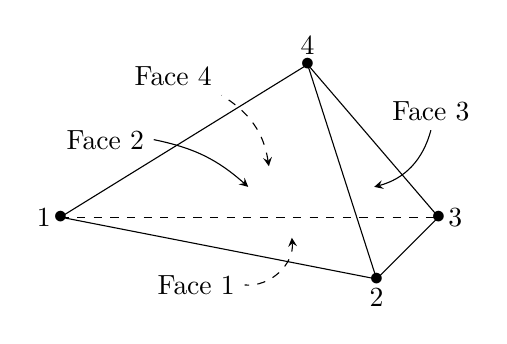
\begin{tikzpicture}[scale=0.6]
					\coordinate (A) at (0,0,0);
					\coordinate (B) at (9,1,6);
					\coordinate (C) at (8,0,0);
					\coordinate (D) at (6,4,2);
					\draw[<-, >=stealth, dashed] (14/3,4/3,2/3) to[bend right=25] ++(-1,1.5,0) node[above left]{Face 4};
					\draw[dashed] (A) node[left]{1} node{$\bullet$} -- (C) node[right]{3} node{$\bullet$};
					\draw[<-, >=stealth, dashed] (17/3,1/3,2) to[bend left=50] ++(-1,-1,0) node[left]{Face 1};
					\draw (A) -- (B) node[below]{2} node{$\bullet$};
					\draw (A) -- (D) node[above]{4} node{$\bullet$};
					\draw (B) -- (C);
					\draw (B) -- (D);
					\draw (C) -- (D);
					\draw[<-, >=stealth] (5,5/3,8/3) to[bend right=15] ++(-2,1,0) node[left]{Face 2};
					\draw[<-, >=stealth] (23/3,5/3,8/3) to[bend right=30] ++(1.2,1.2,0) node[above]{Face 3};
					\end{tikzpicture}}\hspace{2cm}
				\subfloat[\'Elément tétraedrique quadratique à 10 n\oe{}uds - C3D10]{
					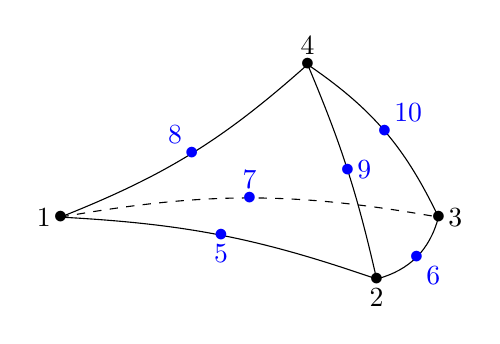
\begin{tikzpicture}[scale=0.6]
					\coordinate (A) at (0,0,0);
					\coordinate (B) at (9,1,6);
					\coordinate (C) at (8,0,0);
					\coordinate (D) at (6,4,2);
					\draw[dashed] (A) node[left]{1} node{$\bullet$} to[bend left=10] node[color=blue,pos=0.5]{$\bullet$} node[color=blue,pos=0.5,above]{7} (C) node{$\bullet$} node[right]{3};
					\draw (A) to[bend left=8] node[color=blue,pos=0.5]{$\bullet$} node[color=blue,pos=0.5,below]{5} (B) node[below]{2} node{$\bullet$};
					\draw (A) to[bend right=10] node[color=blue,pos=0.5]{$\bullet$} node[color=blue,pos=0.5,above left]{8} (D) node[above]{4} node{$\bullet$};
					\draw (B) to[bend right=30] node[color=blue,pos=0.5]{$\bullet$} node[color=blue,pos=0.5,below right]{6} (C);
					\draw (B) to[bend right=5] node[color=blue,pos=0.5]{$\bullet$} node[color=blue,pos=0.5,right]{9} (D);
					\draw (C) to[bend right=15] node[color=blue,pos=0.5]{$\bullet$} node[color=blue,pos=0.5,above right]{10} (D);
					\end{tikzpicture}}
				\caption{\label{fig05:C3D4_C3D10}Définitions des éléments tétraédriques linéaires C3D4 et quadratiques C3D10(M) du logiciel Abaqus.}
			\end{figure}
			Une manière de transformer un élément C3D4 en élément C3D10M est de rajouter un n\oe{}ud sur chaque arrête de l'élément (n\oe{}uds bleus sur la figure \ref{fig05:C3D4_C3D10}). Pour un élément tétraédrique, les n\oe{}uds et les facettes doivent être numérotés de la même manière que sur la figure \ref{fig05:C3D4_C3D10}. Les coordonnées des n\oe{}uds auxiliaires sont calculés par interpolation puis les n\oe{}uds sont renumérotés. Les matrices définissant la liste des n\oe{}uds et des éléments sont ensuite réactualisées.
		\paragraph{Modification du volume maillé\\}
			Afin de modifier la densité apparente du milieu granulaire maillé, il est possible de modifier le volume de chaque grain, sans en changer la géométrie, par homothétie. Pour cela, la position du centre de masse de chaque grain est calculée puis la distance de chaque n\oe{}ud du grain d'origine à son centre de masse est mesurée. Les nouvelles positions des n\oe{}uds sont calculées de telle sorte que la distance entre les nouveaux n\oe{}uds et le centre de masse du grain soit celle mesurée précédemment multipliée par le rapport d'homothétie.
			\\L'objectif ici est de procéder au changement de volume des grains de manière à obtenir la densité apparente mesurée sur les images de tomographie correspondant au volume traité. Pour rappel, la densité apparente est calculée comme le rapport du volume des grains sur le volume total de l'échantillon. Le volume des grains dans l'image est calculé par la mesure du nombre de voxels appartenant aux grains. Le volume des grains maillés est calculé par la somme du volume de chacun des éléments volumiques constituant les grains. Le volume $V_\textrm{ABCD}$ d'un élément tétraédrique de sommets $A$, $B$, $C$ et $D$ est déterminé par l'équation (\ref{eq05:volume_tetraedre}).
			\begin{equation}\label{eq05:volume_tetraedre}
				V_\textrm{ABCD} = \cfrac{1}{6}\times\lvert \det\left( \overrightarrow{AB}, \overrightarrow{AC}, \overrightarrow{AD} \right)\rvert
			\end{equation}
			La densité relative cible à atteindre est celle mesurée par l'intermédiaire de l'image seuillée. Le processus de changement de volume des grains maillés pour atteindre la densité cible est réalisé en deux phases :
			\begin{itemize}
				\item Chaque grain est analysé individuellement de manière à ce que chaque volume maillé soit très proche du volume du grain segmenté. Un processus itératif est mis en \oe{}uvre pour cela. Le volume maillé est d'abord mesuré puis comparé au volume segmenté. Si l'erreur relative sur le volume est inférieure à \SI{0.1}{\percent} alors les deux volumes sont considérés comme égaux. Autrement, une homothétie est réalisée de manière à se rapprocher du volume segmenté. Le processus est répété jusqu'à ce que la tolérance de \SI{0.1}{\percent} soit vérifiée. Cette phase vise à corriger les changements de volume qui apparaissent durant la génération du maillage.
				\item Tous les grains sont analysés de manière à ce que le volume total des grains maillés soit le même que le volume total des zones seuillées sur l'image binaire. Un nouveau processus itératif est mis en place. Les deux volumes sont comparés, si l'écart relatif est supérieur à une valeur de tolérance de \SI{0.1}{\percent} alors une homothétie de l'ensemble des grains est réalisée afin de réduire cet écart. Lorsque l'écart relatif devient inférieur à la tolérance le processus prend fin et les densités sont considérées comme identiques. Dans cette phase, l'objectif est de corriger la densité apparente du milieu qui s'est retrouvée modifiée suite aux étapes de segmentation.
			\end{itemize}
			Au terme de ces phases, le milieu constitué des grains maillés a une densité identique à celle mesurée grâce à la tomographie. Il y a cependant un problème qui peut se manifester : lorsque les grains maillés restent dans leur position d'origine (centres de masse invariants), les grains peuvent s'interpénétrer en certaines zones à cause de l'augmentation du volume. Les longueurs d'interpénétration sont de l'ordre du dixième de voxel. Ces problèmes sont résolus lors de l'intégration des grains dans le programme Abaqus (cf. paragraphe \ref{para05:abaqus}).

\section{Introduction des grains dans un code éléments finis}
	Une fois que les grains sont reconnus individuellement grâce à la segmentation et maillés correctement par l'intermédiaire de la génération du maillage volumique, il est possible d'utiliser un code éléments finis pour simuler la réponse mécanique de l'ensemble de grains à une sollicitation bien définie. Cela ne suffit cependant pas pour pouvoir procéder à des calculs de simulation. Il est encore nécessaire de créer un modèle de simulation pour le programme Abaqus, de définir les conditions aux limites sur le milieu numérisé mais aussi de préparer les résultats à sauvegarder en fin de simulation. Cette partie à pour objectif de présenter l'ensemble de ces éléments. En raison de la complexité et du grand nombre de tâches réalisées pour générer un fichier de modèle Abaqus, le lecteur intéressé est invité à lire la documentation du programme \citep{abaqus2016} pour les parties concernées. L'annexe \ref{annexe:modele_abaqus} présente plus en détail les étapes de génération du modèle de simulation utilisées dans les travaux de cette thèse en illustrant les différentes tâches par des échantillons de script.
	\subsection{Création d'un modèle Abaqus}\label{para05:abaqus}
		Un modèle de simulation Abaqus est constitué de différentes parties. C'est grâce à ce modèle que le programme est capable d'interagir avec les géométries maillées, de connaître leurs propriétés, de soumettre une sollicitation à ces géométries et de savoir quels éléments enregistrer. Le modèle Abaqus, qui est un fichier numérique d'extension ".inp", est un fichier de type texte qui peut être créé à partir de l'interface utilisateur du programme. Cependant, pour des raisons pratiques, il a été choisi de générer ce fichier par l'intermédiaire du script qui traite l'ensemble des données numériques dans ces travaux. En effet, il est aisé de générer un fichier texte à partir d'un script Python ou Matlab qui traite dans le même temps les processus de segmentation, de maillage mais qui peut aussi accéder aux données issues de la corrélation de volume définissant le champ cinématique local (cf. paragraphes \ref{para04:cinematique}, \ref{para05:segmentation} et \ref{para05:maillage}). Les différentes étapes de la création du modèle sont décrites dans les parties qui suivent.
		\subsubsection{Introduction des grains maillés}
			Une première étape consiste à reproduire les grains dans le programme à partir du maillage déjà réalisé. Il est en effet indispensable de définir chaque n\oe{}ud et chaque élément de chacun des grains afin de pouvoir interagir avec ces derniers. Pour cela, chaque grain va être enregistré comme une entité appelée "part". Pour chacune des parts, les n\oe{}uds et les éléments sont définis à partir de la liste des éléments et de la table de connectivité construites lors de la phase de maillage. L'unité de longueur utilisée lors des phases de traitement d'image et de maillage est le voxel et, pour des raisons pratiques, les longueurs sont converties en millimètres dans la simulation. Cette conversion est réalisée en multipliant les coordonnées des n\oe{}uds par la taille d'un voxel en millimètre : $\SI{1}{\voxel} = \SI{0.009}{\milli\meter}$.
			\\Les n\oe{}uds du maillage dans Abaqus sont définis de la même manière que dans \textit{iso2mesh} puisque les repères spatiaux des deux programmes sont tous deux orientés selon les directions de la reconstruction de tomographie. Seule la conversion d'unité de longueur est réalisée. La table de connectivité de chacun des grains reste inchangée.
		\subsubsection{Définition du matériau}
			La géométrie des grains est importée mais cela ne suffit pas pour le code éléments finis. Il est également important de fournir l'information sur le comportement physique du matériau constituant les grains, à savoir de polystyrène. Une masse volumique est déterminée à partir de \citet{wypych_handbook_2016} : elle vaut ici \SI{1.05}{\gram\per\centi\meter\cubed}. Dans cette thèse, le comportement mécanique du matériau suit le modèle élastoplastique de Von Mises avec écrouissage isotrope. Une illustration de ce comportement est donnée par la courbe de charge linéaire présentée sur la figure \ref{fig05:PS_comportement}. Ce modèle permet de tenir compte des déformations irréversibles des grains dans les zones de fortes contraintes. Un écrouissage, isotrope puisqu'il ne dépend \textit{a priori} pas du chemin de chargement, est défini afin de modéliser le durcissement du polystyrène pour des déformations relativement grandes.
			\\Le choix d'un comportement simplement élasto-plastique sans influence de la vitesse de déformation s'explique essentiellement par des raisons pratiques. Premièrement, les vitesses de sollicitations étant faibles il a été choisi dans une première approche d'ignorer les effets visqueux, bien qu'ils soient observables sur les essais expérimentaux (quoiqu'il ait été impossible de séparer la contribution de la cellule triaxiale en PMMA et celle des grains de polystyrène eux-mêmes). Deuxièmement, pour des raisons numériques cette fois, il est difficile de se passer de la plasticité car celle-ci permet d'éviter les concentrations de contraintes dans les zones de contact. C'est également pour faciliter la convergence du calcul qu'un comportement écrouissable et non parfaitement plastique a été choisi.
			\\Les propriétés mécaniques retenues pour renseigner le comportement plastique sont la limite élastique du polystyrène issue de \citet{wypych_handbook_2016}, à savoir \SI{45}{\mega\pascal}, et un module d'écrouissage de \SI{8.3}{\mega\pascal}.
			\begin{figure}\centering
				\includegraphics[width=0.7\textwidth]{plastic_curve.eps}
				\caption{\label{fig05:PS_comportement}Courbes déterminant le comportement du matériau polystyrène.}
			\end{figure}
		\subsubsection{Assemblage}
			Dans l'étape précédente, les grains maillés ont été introduits indépendamment les uns des autres en utilisant les coordonnées des n\oe{}uds obtenues lors du maillage avec iso2mesh. Pour ces raisons, les coordonnées enregistrées précédemment sont celles calculées à partir d'origines différentes (une origine différente pour chaque grain). Les coordonnées obtenues lors du maillage sont en fait calculées à partir de l'origine, locale, de l'image fournie au mailleur. Cette origine locale est donc le sommet du premier voxel rencontré dans chacune des directions de l'image 3D - un sommet du parallélépipède qui englobe tout le grain. L'objectif étant de simuler un milieu granulaire, il est obligatoire de représenter l'ensemble des grains dans un même espace, et de manière correcte. L'étape d'assemblage est là pour cela. Lors de l'étape d'assemblage, il est nécessaire de définir une origine, globale, qui soit commune à tous les grains de manière à pouvoir les situer correctement l'un par rapport à l'autre. Une méthode pour cela est de générer des repères locaux pour chacun des grains. L'ensemble du repère local et du part associé au grain est appelé "instance". Il faut ensuite considérer, pour chaque grain, le vecteur position de l'origine locale dans l'image segmentée dans le but de procéder à une translation de l'instance suivant ce même vecteur. Dans ce cas, l'origine du repère global sera identique à l'origine de l'image segmentée (un des sommets de l'image segmentée). Pour rappel, la position des repères locaux est enregistrée à la fin de la phase de segmentation (cf. paragraphe \ref{para05:post_segm}). La figure \ref{fig05:assemblage_abaqus} permet d'observer un assemblage de grain dans Abaqus.
			\begin{figure}\centering
				\includegraphics[width=0.95\textwidth]{sample_before.png}
				\caption{\label{fig05:assemblage_abaqus}Assemblage des grains maillés constituant un échantillon numérique du milieu granulaire étudié. Ce volume est constitué de \num{253} grains.}
			\end{figure}
		\subsubsection{Définition des surfaces}
			Les grains sont correctement reconnus et positionnés par Abaqus. Il reste encore à identifier correctement les surfaces de manière à pouvoir définir des paires de surfaces qui rentreront potentiellement en contact pendant le calcul de simulation. Il est primordial de définir l'orientation des facettes de chaque élément en surface des grains de manière à ce que la normale des facettes soit dirigée vers l'extérieur. La figure \ref{fig05:C3D4_C3D10} indique la numérotation des faces d'un élément tétraédrique. Une façon de s'assurer que les surfaces soient bien définies et orientées est de créer des listes d'éléments, pour chaque grain, en fonction des facettes qui caractérisent la surface des grains. Ainsi, chaque grain a quatre listes : une liste indiquant les éléments pour lesquels la face 1 est une surface libre du grain, une pour laquelle les faces 2 des éléments sont sur la surface du grains, de même pour les faces 3 et 4. La surface totale du grain est définie par la réunion de ces quatre listes. D'un point de vue pratique, cela est rendu possible grâce à la sauvegarde des éléments surfaciques qui a été faite lors du maillage (cf. paragraphe \ref{para05:post_segm}). En effet, en connaissant la liste des n\oe{}uds caractérisant la surface libre du grain et en analysant chaque élément tétraédrique du grain, il est possible de savoir si les éléments possèdent une ou plusieurs face(s) sur la frontière extérieure du grain ou non, et si oui selon laquelle (lesquelles).
		\subsubsection{Définition des contacts}
			Lorsqu'ils vont se déplacer et se déformer lors de la simulation, les grains vont entrer en contact avec d'autres grains voisins. Une étape consiste donc à déterminer les interactions propres à ces contacts. Les contacts à considérer dans les calculs numériques sont des contacts entre des éléments dont le matériau constitutif est le même, à savoir le polystyrène. La littérature \citep{engineeringtoolbox,matweb,wypych_handbook_2016} indique un coefficient de friction de \num{0.5} pour des essais de frottement entre deux surfaces en polystyrène. L'utilisation de ce coefficient dans une loi de Coulomb permet de déterminer les efforts tangentiels à la surface de contact en fonction des efforts normaux. Aucune cohésion de contact n'est introduite.
			\\L'algorithme de modélisation des  contacts utilisé dans Abaqus est l'algorithme "general contact" qui est bien plus efficace en terme de temps de calcul que l'algorithme "contact pairs" \citep{abaqus2016}. Les contacts sont définis comme rigides : la pression de contact d'une surface sur une autre n'existe pas tant que la distance qui sépare ces deux surfaces est positive. Dans le cas où cette distance devient négative, des efforts de contact proportionnels à la distance apparaissent.
			\\Une fois que les contacts sont définis correctement, il est important d'indiquer au code éléments finis les couples de surfaces pour lesquelles des contacts peuvent survenir. Sans cela, le programme considère par défaut toutes les interactions possibles entre surfaces et le calcul devient alors très lent. Pour chaque grain, il a été choisi de ne considérer des contacts potentiels qu'avec les grains distant de moins de \SI{180}{\micro\meter} (ou encore \SI{20}{\voxel} sur les images 3D), soit une distance légèrement plus grande que la taille d'un grain moyen. Si deux grains, dans l'état initial, sont distants l'un de l'autre de plus de \SI{180}{\micro\meter} alors aucun contact entre ces deux grains n'existera. La distance de \SI{20}{\voxel} est justifiée puisqu'aucun cas de grains superposés n'a été visualisé dans ces travaux.
		\subsubsection{Correction des contacts initiaux}
			Lors de l'analyse et de la correction du maillage (cf. paragraphe \ref{para05:maillage_correction}), le volume des grains est généralement augmenté volontairement de manière à ce que la densité apparente du milieu numérisé soit identique à celle du milieu observé par tomographie. En augmentant le volume des grains mais en conservant leur position d'origine, certains grains voisins peuvent s'interpénétrer en certaines zones en raison des différentes opérations affectant la géométrie des grains lors du traitement d'image et du maillage, en particulier le lissage des surfaces. Ce cas est illustré sur la figure \ref{fig05:contact_correction}-(a). Ces zones sont très certainement des zones de contacts entre ces mêmes grains dans l'échantillon réel. Cependant, le fait que certains éléments tétraédriques issus de différents grains s'interpénètrent pose des problèmes dès le départ de la simulation. En effet, les contacts ne sont pas correctement établis dans les régions concernées. Pour des raisons d'optimisation du temps de calcul, les contacts ne sont considérés que lorsque la distance n\oe{}ud-facette entre deux surfaces en contact est inférieure à un seuil donné par défaut. Si les n\oe{}uds des surfaces de contact sont plus éloignés que la distance seuil (vers l'intérieur ou vers l'extérieur) ils ne sont plus pris en compte et les forces nodales de contact sont annulées.
			\\Le programme Abaqus possède une fonction qui permet de corriger ces défauts en modifiant directement les coordonnées des n\oe{}uds situés à l'intérieur d'un élément ou bien en créant un "offset", c'est-à-dire que la distance n\oe{}ud-facette pour le calcul du contact est artificiellement décalée de sorte à ce que la distance nulle corresponde à la configuration initiale. Ainsi les n\oe{}uds des surfaces en contact ont une force initialement nulle, même s'il y a une légère interpénétration. Dans les travaux présentés, il a été choisi de ne pas modifier directement la position des n\oe{}uds constituant des éléments interpénétrés mais de considérer des offsets lors du calcul des forces. La recherche des contacts n\oe{}ud-facette initiaux est réalisée à une certaine distance à l'intérieur des grains (figure \ref{fig05:contact_correction}-(b)) et à l'extérieur (figure \ref{fig05:contact_correction}-(c)) afin que le logiciel Abaqus considère la surface de contact corrigée (figure \ref{fig05:contact_correction}-(d)). La zone de recherche des contacts n\oe{}uds-facette à l'intérieur des grains et de \SI{10}{\micro\meter}, soit légèrement plus qu'un voxel ; celle à l'extérieur des grains est de \SI{4}{\micro\meter}, soit légèrement moins de la moitié d'un voxel. La correction des contacts vers l'extérieur des surfaces a pour objectif de générer des contacts lorsque les distances sont très faibles entre les éléments (moins d'un voxel dans l'image segmentée). Cela permet d'assurer que les efforts sont transmis de grain en grain dès le départ de la simulation.
			\begin{figure}\centering
				~\hfill
				\subfloat[Contact avec interpénétration des éléments]{
					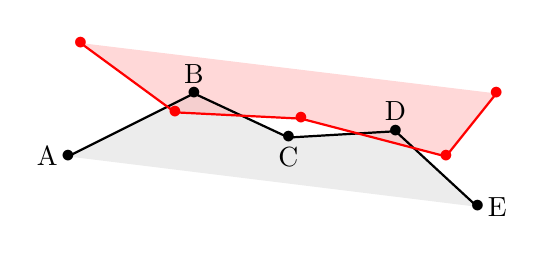
\begin{tikzpicture}[scale=0.8]
						\coordinate (A0) at (0,0);
						\coordinate (A1) at (2,1);
						\coordinate (A2) at (3.5,0.3);
						\coordinate (A3) at (5.2,0.4);
						\coordinate (A4) at (6.5,-0.8);
						\coordinate (B0) at (0.2,1.8);
						\coordinate (B1) at (1.7,0.7);
						\coordinate (B2) at (3.7,0.6);
						\coordinate (B3) at (6,0);
						\coordinate (B4) at (6.8,1);
						\fill[gray!30, opacity=0.5] (A0) node{$\bullet$} -- (A1) node{$\bullet$} -- (A2) node{$\bullet$} -- (A3) node{$\bullet$} -- (A4) node{$\bullet$};
						\fill[red!30, opacity=0.5] (B0) node{$\bullet$} -- (B1) node{$\bullet$} -- (B2) node{$\bullet$} -- (B3) node{$\bullet$} -- (B4) node{$\bullet$};
						\draw[thick] (A0) node{$\bullet$} node[left]{A} -- (A1) node{$\bullet$} node[above]{B} -- (A2) node{$\bullet$} node[below]{C} -- (A3) node{$\bullet$} node[above]{D} -- (A4) node{$\bullet$} node[right]{E};
						\draw[red, thick] (B0) node{$\bullet$} -- (B1) node{$\bullet$} -- (B2) node{$\bullet$} -- (B3) node{$\bullet$} -- (B4) node{$\bullet$};
					\end{tikzpicture}}\hfill
				~\hfill
				\subfloat[Recherche des n\oe{}uds à l'intérieur des grains]{
					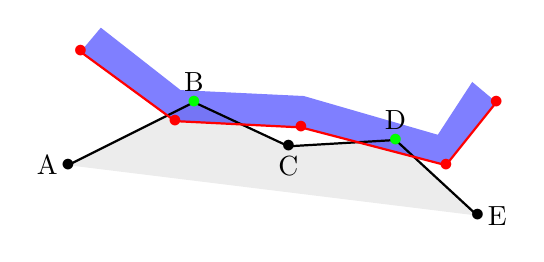
\begin{tikzpicture}[scale=0.8]
						\pgfmathsetmacro{\rayon}{0.5}
						\coordinate (A0) at (0,0);
						\coordinate (A1) at (2,1);
						\coordinate (A2) at (3.5,0.3);
						\coordinate (A3) at (5.2,0.4);
						\coordinate (A4) at (6.5,-0.8);
						\coordinate (B0) at (0.2,1.8);
						\coordinate (B1) at (1.7,0.7);
						\coordinate (B2) at (3.7,0.6);
						\coordinate (B3) at (6,0);
						\coordinate (B4) at (6.8,1);
						\coordinate (B0bis) at ({0.2+\rayon*cos(50)}, {1.8+\rayon*sin(50)});
						\coordinate (B1bis) at ({1.7+\rayon*cos(80)}, {0.7+\rayon*sin(80)});
						\coordinate (B2bis) at ({3.7+\rayon*cos(85)}, {0.6+\rayon*sin(85)});
						\coordinate (B3bis) at ({6+\rayon*cos(180-75)}, {0+\rayon*sin(180-75)});
						\coordinate (B4bis) at ({6.8+\rayon*cos(180-40)}, {1+\rayon*sin(180-40)});
						\fill[gray!30, opacity=0.5] (A0) node{$\bullet$} -- (A1) node{$\bullet$} -- (A2) node{$\bullet$} -- (A3) node{$\bullet$} -- (A4) node{$\bullet$};
						\fill[blue, opacity=0.5] (B0bis) -- (B1bis) -- (B2bis) -- (B3bis) -- (B4bis) -- (B4) -- (B3) -- (B2) -- (B1) -- (B0) -- cycle;
						\draw[thick] (A0) node{$\bullet$} node[left]{A} -- (A1) node[green]{$\bullet$} node[above]{B} -- (A2) node{$\bullet$} node[below]{C} -- (A3) node[green]{$\bullet$} node[above]{D} -- (A4) node{$\bullet$} node[right]{E};
						\draw[red, thick] (B0) node{$\bullet$} -- (B1) node{$\bullet$} -- (B2) node{$\bullet$} -- (B3) node{$\bullet$} -- (B4) node{$\bullet$};
					\end{tikzpicture}}\hfill~\\
				~\hfill
				\subfloat[Recherche des n\oe{}uds à l'intérieur des grains]{
					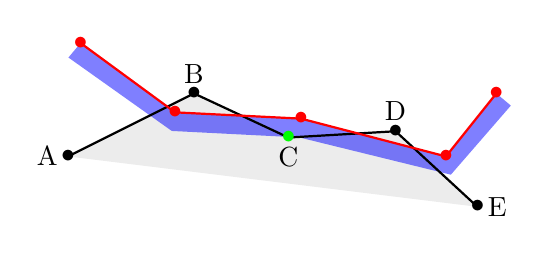
\begin{tikzpicture}[scale=0.8]
						\pgfmathsetmacro{\rayon}{0.3}
						\coordinate (A0) at (0,0);
						\coordinate (A1) at (2,1);
						\coordinate (A2) at (3.5,0.3);
						\coordinate (A3) at (5.2,0.4);
						\coordinate (A4) at (6.5,-0.8);
						\coordinate (B0) at (0.2,1.8);
						\coordinate (B1) at (1.7,0.7);
						\coordinate (B2) at (3.7,0.6);
						\coordinate (B3) at (6,0);
						\coordinate (B4) at (6.8,1);
						\coordinate (B0bis) at ({0.2+\rayon*cos(180+50)}, {1.8+\rayon*sin(180+50)});
						\coordinate (B1bis) at ({1.7+\rayon*cos(180+80)}, {0.7+\rayon*sin(180+80)});
						\coordinate (B2bis) at ({3.7+\rayon*cos(180+85)}, {0.6+\rayon*sin(180+85)});
						\coordinate (B3bis) at ({6+\rayon*cos(-75)}, {0+\rayon*sin(-75)});
						\coordinate (B4bis) at ({6.8+\rayon*cos(-40)}, {1+\rayon*sin(-40)});
						\fill[gray!30, opacity=0.5] (A0) node{$\bullet$} -- (A1) node{$\bullet$} -- (A2) node{$\bullet$} -- (A3) node{$\bullet$} -- (A4) node{$\bullet$};
						\fill[blue, opacity=0.5] (B0bis) -- (B1bis) -- (B2bis) -- (B3bis) -- (B4bis) -- (B4) -- (B3) -- (B2) -- (B1) -- (B0) -- cycle;
						\draw[thick] (A0) node{$\bullet$} node[left]{A} -- (A1) node{$\bullet$} node[above]{B} -- (A2) node[green]{$\bullet$} node[below]{C} -- (A3) node{$\bullet$} node[above]{D} -- (A4) node{$\bullet$} node[right]{E};
						\draw[red, thick] (B0) node{$\bullet$} -- (B1) node{$\bullet$} -- (B2) node{$\bullet$} -- (B3) node{$\bullet$} -- (B4) node{$\bullet$};
					\end{tikzpicture}}\hfill
				\subfloat[Surface de contact corrigée]{
					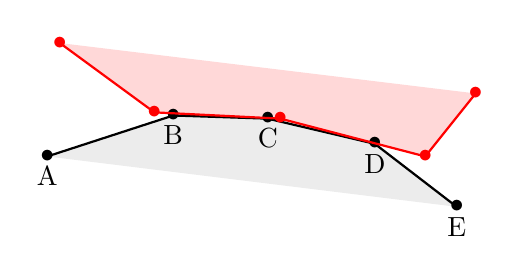
\begin{tikzpicture}[scale=0.8]
						\coordinate (A0) at (0,0);
						\coordinate (A1) at (2,0.65);
						\coordinate (A2) at (3.5,0.6);
						\coordinate (A3) at (5.2,0.2);
						\coordinate (A4) at (6.5,-0.8);
						\coordinate (B0) at (0.2,1.8);
						\coordinate (B1) at (1.7,0.7);
						\coordinate (B2) at (3.7,0.6);
						\coordinate (B3) at (6,0);
						\coordinate (B4) at (6.8,1);
						\fill[gray!30, opacity=0.5] (A0) node{$\bullet$} -- (A1) node{$\bullet$} -- (A2) node{$\bullet$} -- (A3) node{$\bullet$} -- (A4) node{$\bullet$};
						\fill[red!30, opacity=0.5] (B0) node{$\bullet$} -- (B1) node{$\bullet$} -- (B2) node{$\bullet$} -- (B3) node{$\bullet$} -- (B4) node{$\bullet$};
						\draw[thick] (A0) node{$\bullet$} node[below]{A} -- (A1) node{$\bullet$} node[below]{B} -- (A2) node{$\bullet$} node[below]{C} -- (A3) node{$\bullet$} node[below]{D} -- (A4) node{$\bullet$} node[below]{E};
						\draw[red, thick] (B0) node{$\bullet$} -- (B1) node{$\bullet$} -- (B2) node{$\bullet$} -- (B3) node{$\bullet$} -- (B4) node{$\bullet$};
					\end{tikzpicture}}\hfill~
			\caption{\label{fig05:contact_correction}Correction d'une zone de contact pour laquelle une interpénétration des éléments était initialement présente (a). La correction est faite par rapport à la surface rouge. La recherche des contacts n\oe{}ud-facette à l'intérieur (b) et à l'extérieur (c) des grains permet d'identifier le n\oe{}uds à corriger. Les positions des n\oe{}uds B, C et D sont corrigées (d). En réalité la position des n\oe{}uds n'est pas modifiée dans ces travaux mais la distance qui les sépare de la surface de contact corrigée est enregistrée et utilisé en offset dans le calcul des forces de contact.}
			\end{figure}
			
	\subsection{Conditions aux limites}\label{para05:abaqus_BC}
		La géométrie, le matériau et les interactions entre grains dans le milieu granulaire ont été correctement introduits. Une étape supplémentaire est de fournir une information sur les conditions aux limites du milieu. L'objectif ici est de procéder à la simulation de ce qu'il s'est passé lors d'un essai mécanique réel. Il est donc nécessaire de considérer les conditions aux limites les plus proches de celles issues de l'essai réel. Une méthode pour cela, qui est illustrée sur la figure \ref{fig05:conditions_limites}, consiste à piloter en déplacement les grains (en bleu sur la figure) situés dans la zone de pilotage des grains qui n'est autre que la bordure extérieure de l'échantillon numérisé (en rouge sur la figure). Si les déplacements (flèches bleues sur la figure \ref{fig05:conditions_limites}) des grains correspondent à ceux observés en tomographie, la sollicitation du milieu numérique devrait être semblable à celle du milieu expérimental. Afin de piloter les grains en périphérie, il n'est pas avantageux de provoquer le déplacement de l'ensemble des n\oe{}uds du grains pour ne pas engendrer de mouvements de corps rigides sans aucune déformation des grains pilotés, mais surtout pour ne pas surcontraindre l'échantillon : ce qui donnerait lieu à des problèmes numériques (en particulier des concentrations de contrainte au niveau des contacts). Une manière de contourner cela est de créer des n\oe{}uds de référence (points bleus sur la figure \ref{fig05:conditions_limites}) aux centres de masse des grains pilotés, de coupler les n\oe{}uds des grains avec les n\oe{}uds de référence et de piloter le déplacement des n\oe{}uds de référence.
		\begin{figure}\centering
			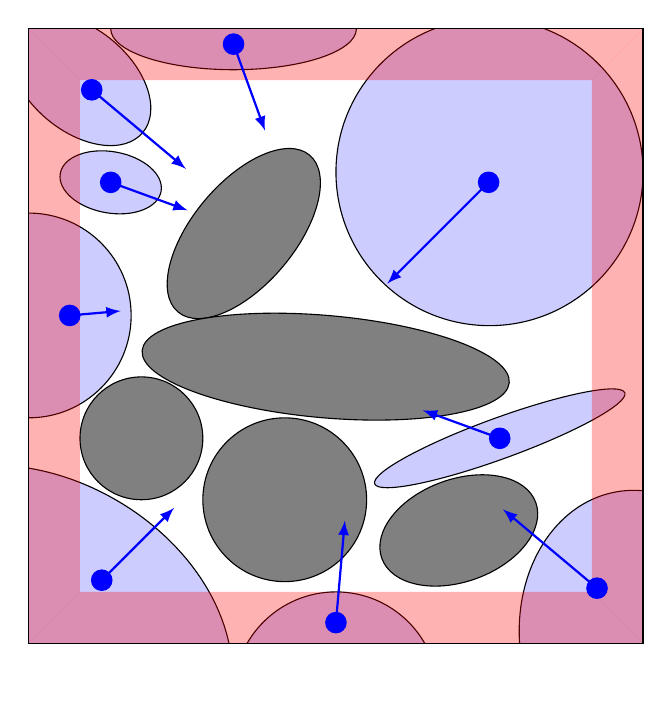
\begin{tikzpicture}[scale=1.3]
			\tikzset{bordure/.style={red, opacity=0.3},
				grain_int/.style={fill=black!50},
				grain_ext/.style={fill=blue!20},
				marqueur/.style={blue},
				deplacement/.style={blue, -latex, thick}}
			% défini les centres des grains
			\coordinate (A) at (2.1,4); \coordinate (B) at (1.1,2); \coordinate (C) at (0.1,0.1);
			\coordinate (D) at (0.8,4.5); \coordinate (E) at (0,3.2); \coordinate (F) at (0.5,5.5);
			\coordinate (G) at (2.9, 2.7); \coordinate (H) at (4.5,4.6); \coordinate (I) at (2.5, 1.4);
			\coordinate (J) at (2,6); \coordinate (K) at (4.6,2); \coordinate (L) at (6,0);
			\coordinate (M) at (4.2,1.1); \coordinate (N) at (3,-0.5);
			% dessine les grains
			\begin{scope}
			\clip (0,0) rectangle (6,6);
			\filldraw[grain_int, rotate=50] (A) ellipse (1 and 0.5);
			\filldraw[grain_int] (B) circle (0.6);
			\filldraw[grain_ext, rotate=-30] (C) ellipse (2 and 1.5);
			\filldraw[grain_ext, rotate=-10] (D) ellipse (0.5 and 0.3);
			\filldraw[grain_ext] (E) circle (1);
			\filldraw[grain_ext, rotate=-40] (F) ellipse (0.8 and 0.5);
			\filldraw[grain_int, rotate=-5] (G) ellipse (1.8 and 0.5);
			\filldraw[grain_ext] (H) circle (1.5);
			\filldraw[grain_int] (I) circle (0.8);
			\filldraw[grain_ext, rotate=0] (J) ellipse (1.2 and 0.4);
			\filldraw[grain_ext, rotate=20] (K) ellipse (1.3 and 0.2);
			\filldraw[grain_ext, rotate=-80] (L) ellipse (1.5 and 1.2);
			\filldraw[grain_int, rotate=20] (M) ellipse (0.8 and 0.5);
			\filldraw[grain_ext] (N) circle (1);
			\end{scope}
			% dessine la bordure
			\fill[bordure] (0,6) -- (0,0) -- (0.5,0.5) -- (0.5,5.5);
			\fill[bordure] (0,6) -- (6,6) -- (5.5,5.5) -- (0.5,5.5);
			\fill[bordure] (6,6) -- (6,0) -- (5.5,0.5) -- (5.5,5.5);
			\fill[bordure] (6,0) -- (0,0) -- (0.5,0.5) -- (5.5,0.5);
			% dessine les centres de masse
			\filldraw[marqueur] (C) ++(40:0.8) circle (0.1); \draw[deplacement] (C) ++(40:0.8) -- ++(45:1);
			\filldraw[marqueur] (D) circle (0.1); \draw[deplacement] (D) -- ++(-20:0.8);
			\filldraw[marqueur] (E) ++(0:0.4) circle (0.1); \draw[deplacement] (E) ++(0:0.4) -- ++(5:0.5);
			\filldraw[marqueur] (F) ++(-40:0.15) circle (0.1); \draw[deplacement] (F) ++(-40:0.15) -- ++(-40:1.2);
			\filldraw[marqueur] (H) ++(-95:0.1) circle (0.1); \draw[deplacement] (H) ++(-95:0.1) -- ++(-135:1.4);
			\filldraw[marqueur] (J) ++(-90:0.15) circle (0.1); \draw[deplacement] (J) ++(-90:0.15) -- ++(-70:0.9);
			\filldraw[marqueur] (K) circle (0.1); \draw[deplacement] (K) -- ++(160:0.8);
			\filldraw[marqueur] (L) ++(130:0.7) circle (0.1); \draw[deplacement] (L) ++(130:0.7) -- ++(140:1.2);
			\filldraw[marqueur] (N) ++(90:0.7) circle (0.1); \draw[deplacement] (N) ++(90:0.7) -- ++(85:1.);
			% dessine le cadre
			\draw (0,0) rectangle (6,6);
			% trouver les points ---- a cacher pour la version finale
			%\draw (A) node{A}; \draw (B) node{B}; \draw (C) node{C}; \draw (D) node{D};
			%\draw (E) node{E}; \draw (F) node{F}; \draw (G) node{G}; \draw (H) node{H};
			%\draw (I) node{I}; \draw (J) node{J}; \draw (K) node{K}; \draw (L) node{L};
			%\draw (M) node{M}; \draw (N) node{N};
			\end{tikzpicture}
			\caption{\label{fig05:conditions_limites}Schématisation du principe de pilotage des grains en déplacement. Une bordure est définie sur la frontière extérieure de l'échantillon numérique (zone rouge transparente). Tous les grains dont au moins une partie est dans cette bordure (grains bleus clairs) sont pilotés en déplacement. Les déplacements imposés (flèches bleues) aux centres de masse des grains dans l'échantillon (points bleus) sont ceux observés par interpolation linéaire des résultats de corrélation de volumes.}
		\end{figure}
		\subsubsection{Création des n\oe{}uds de référence}
			Le n\oe{}ud de référence ne fait pas partie du maillage. Il s'agit d'un point qui est rajouté au modèle pour faciliter le pilotage des grains en déplacement. C'est en quelque sorte un n\oe{}ud virtuel. Une bordure de quelques voxels, appelée "zone de pilotage des grains" et représentée en transparence rouge sur la figure \ref{fig05:conditions_limites}, est définie de manière à repérer les grains qui vont être pilotés. Tous les grains qui sont inclus, au moins en partie, dans cette bordure sont considérés comme des grains périphériques et seront pilotés en déplacement. Ainsi, pour chacun de ces grains, un n\oe{}ud de référence est créé au centre de masse de ceux-ci située dans la bordure afin de créer un élément "pilotable". Les n\oe{}uds de référence sont créés dans l'assemblage de la même manière que pour un n\oe{}ud de maillage.
		\subsubsection{Couplage avec les n\oe{}uds de référence}
			Les n\oe{}uds de référence ont été créés de manière à pouvoir être pilotés en déplacement. Afin que le déplacement du n\oe{}ud permette le déplacement d'un ensemble de n\oe{}uds voisins, un couplage est défini. Le couplage utilisé dans ces travaux permet de contrôler, par l'intermédiaire d'une méthode de pondération, la transmission des efforts et des moments n\oe{}ud à n\oe{}ud à partir du point de référence. Alors que le point de référence est contraint en déplacement, les n\oe{}uds couplés à cette référence sont contraints en force puisque l'ensemble des efforts et moments exercés sur le point de référence est distribué aux n\oe{}uds couplés avec ce de dernier. Pour permettre un tel couplage, une zone d'influence ainsi qu'un profil de distribution des forces et des moments doivent être déterminés. La zone d'influence correspond à la zone dans laquelle les n\oe{}uds vont être couplés avec la référence. Il s'agit d'une sphère centrée sur le n\oe{}ud de référence. Le rayon de cette sphère a été choisi à \SI{50}{\micro\meter} soit près d'un tiers de la taille d'un grain moyen. Les coefficients de pondération des n\oe{}uds du maillage couplés avec la référence vont dépendre de la distance par rapport au point de référence $r_i$ et du rayon maximal $r_\textrm{max}$ qui est le rayon de la sphère précédemment établie. Le profil de distribution des efforts est cubique par rapport à la distance au point de référence et permet, par rapport à un profil linéaire, de donner plus d'importance au n\oe{}uds proches de la référence et moins d'importance à ceux qui en sont les plus distants. La zone d'influence ainsi que le profil de distribution sont représentés sur la figure \ref{fig05:couplage}.
			\begin{figure}\centering
				\subfloat[Grain maillé et ensemble des n\oe{}uds couplés à la référence.]{\includegraphics[width=.48\textwidth]{coupling_273.eps}}\hfill
				\subfloat[Valeur du coefficient de pondération pour le couplage distributif en fonction de la distance à la référence.]{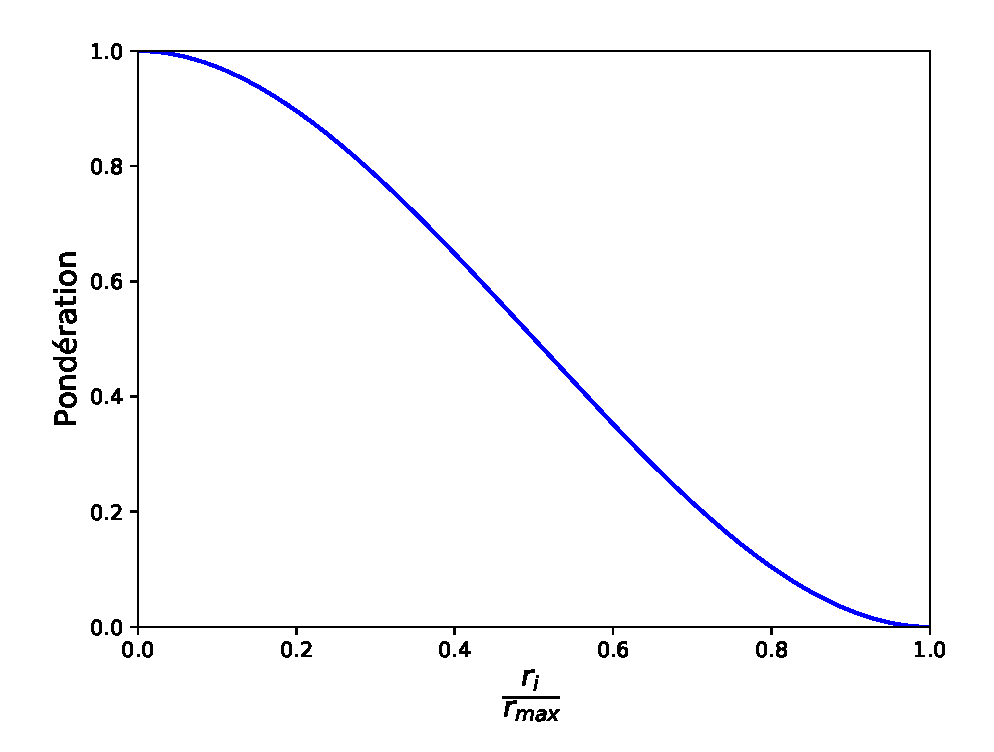
\includegraphics[width=.45\textwidth]{coupling_cibique_fr.eps}}
				\caption{\label{fig05:couplage}(a) Zone d'influence et (b) profil de distribution pour le couplage d'un grain à son n\oe{}ud de référence.}
			\end{figure}
		\subsubsection{Pilotage des n\oe{}uds de référence}
		Lorsque les couplages ont bien été définis, il est possible d'imposer une sollicitation aux n\oe{}uds de référence pour imposer un déplacement des grains en périphérie. Les déplacements imposés sont définis à partir des déplacements mesurés en corrélation d'images (cf. paragraphe \ref{para04:cinematique}). L'amplitude des déplacements est déterminée par interpolation linéaire 3D du champ de déplacement mesuré. On notera que le déplacement mesuré par DVC est un déplacement associé à une fenêtre de corrélation dont la dimension est supérieure à la dimension d'un grain. Ainsi le déplacement appliqué, dans la simulation, à un seul grain est le déplacement mesuré moyenné sur plusieurs grains (faute d'être capable, pour l'instant, de mesurer directement le déplacement d'un grain expérimental, ou encore mieux, de son centre de masse). Cette méthode implique une approximation au niveau de l'application des déplacements imposés, approximation qui ne pourra être satisfaisante qu'en impliquant dans la simulation un assez grand nombre de grains.
		\begin{figure}\centering
			\subfloat[]{
				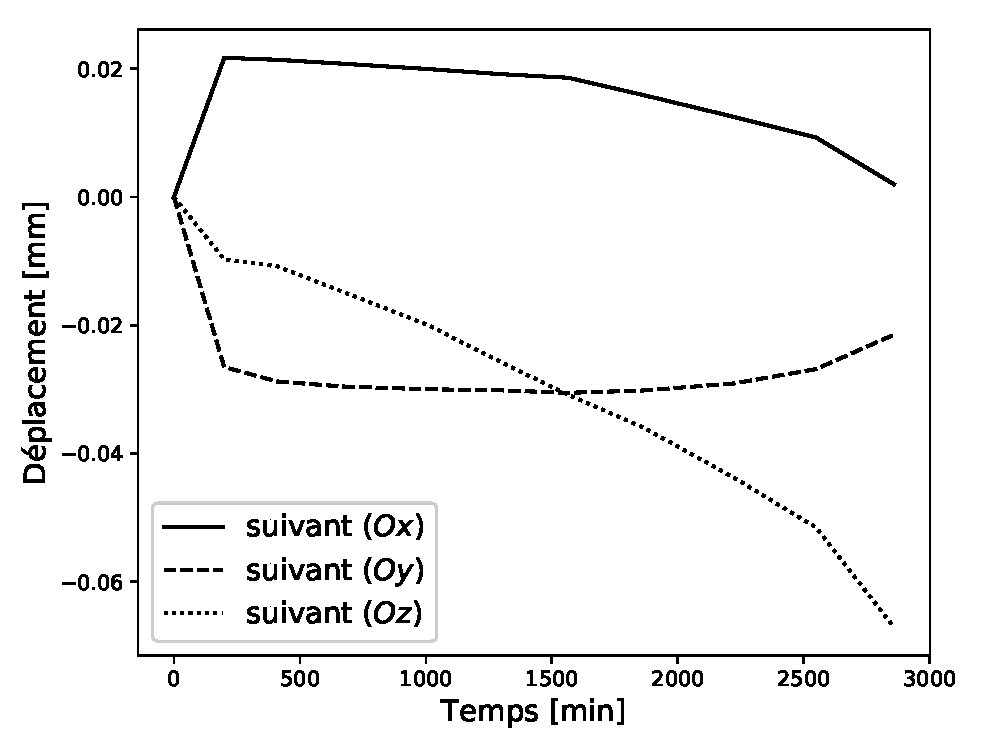
\includegraphics[width=.45\textwidth]{amplitude/courbes_amplitude.eps}}\hfill
			\subfloat[]{
				\includegraphics[width=.45\textwidth]{amplitude/courbes_amplitude_smooth.eps}}
			\caption{\label{fig05:courbes_amplitude}Courbes de déplacement d'un n\oe{}ud de référence (a) mesurées mais linéaires par partie et (b) approximées mais régularisées.}
		\end{figure}
		\\Les vitesses de chargement dans Abaqus sont considérées identiques aux vitesses de chargement expérimentales puisque les courbes d'amplitude du déplacement sont définies avec les temps observés dans l'expérience. Les positions des grains varient de manière linéaire dans le temps entre les positions connues aux différents états de chargement grâce à la tomographie. La position est donc une fonction linéaire par partie du temps : cela veut dire que certains points sont singuliers. La présence de points singuliers dans l'évolution de la position au cours du temps engendre des discontinuités de la vitesse et pose un problème dans les calculs car l'accélération (en principe infinie aux points singuliers) va présenter des sauts dont l'ampleur dépend du pas de temps. Or l'accélération est utilisée pour résoudre l'équation fondamentale du mouvement dans le calcul ($Kx = F - M\ddot{x}$). Pour remédier à cela, une courbure est créée au niveau des points singuliers de manière à régulariser l'évolution de la position avec le temps. La figure \ref{fig05:courbes_amplitude} montre un exemple du lissage de la position en fonction du temps.
		\\Le choix d'un schéma d'intégration explicite concernant la simulation rend possible la création de forces d'inertie avec le déplacement des grains. Cet effet est d'autant plus marqué qu'un processus de modification de la masse des grains ("mass scaling" dans Abaqus) est réalisé afin de permettre l'augmentation des incréments lors du chargement mécanique. Une manière de s'assurer que les forces d'inertie sont négligeables devant les forces de contact dans le milieu granulaire est d'analyser les courbes de l'énergie cinétique et de l'énergie totale du système au cours du temps et de les comparer. Pour l'ensemble des essais réalisés dans cette thèse, le coefficient de "mass scaling" a été choisi de manière à rendre l'amplitude de l'énergie cinétique négligeable devant celle de l'énergie totale.
	\subsection{\'Eléments de sortie}
		L'ensemble des éléments permettant de procéder à la simulation a été fourni dans le modèle Abaqus. Il reste cependant encore quelques éléments à introduire dans le modèle afin de pouvoir traiter les données de simulation en fin de tâche. En effet, il est nécessaire de fournir une liste de types de données à sauvegarder.
		\\En vue du nombre de degrés de liberté dans une simulation de quelques centaines de grains et du nombre de simulation à mener, il est primordial de sauver de l'espace disque et de rendre plus fluide le processus de traitement des données. Pour cela il a été choisi de sauvegarder le minimum de données utiles au post-traitement des simulations. Dans ce but, un minimum de champs vectoriels et scalaires sont enregistrés et, notamment, les champs de contrainte et de déformation ne sont pas enregistrés du fait de l'importance du volume qu'ils occupent. Finalement, il a été choisi de sauvegarder uniquement :
		\begin{itemize}
			\item Le champ de déplacement. Cela permet de connaître la position de chaque n\oe{}ud à tout moment dans la simulation et donc de connaître directement les états déformés du milieu granulaire.
			\item Pour chaque contact, la force totale liée à la pression de contact et les contraintes de friction.
			\item Pour chaque n\oe{}ud de référence, le torseur lié aux efforts de réaction.
			\item Pour chaque grain, la position du centre de masse, le déplacement du centre de masse et la masse totale.
		\end{itemize}
	\paragraph{}
		Ce manuscrit présente au chapitre \ref{chap:couplage} une campagne de calculs menés en série visant à reproduire, à l’échelle mésoscopique, les évolutions mesurées durant la compression triaxiale de révolution. Sur la base d’un jeu de paramètres dédiés au comportement intra et inter-granulaire, l’objectif a donc été d’identifier un jeu de paramètres quantitatif conduisant à reproduire au mieux la réponse expérimentale. De sorte à aboutir aux résultats de synthèse présentés au chapitre \ref{chap:couplage}, il a été nécessaire de construire et post-traiter un ensemble composé d’une centaine de cas de simulation.

\section{Campagnes de simulation}
	\begin{figure}\centering
	\begin{tikzpicture}[scale=1.]
		\tikzset{debutfin/.style={ellipse, draw},
				 condition/.style={diamond, draw},
			 	 etape/.style={rectangle, rounded corners=4pt, draw, text width=6cm, text centered},
		 	 	 consequence/.style={rectangle, draw, fill=gray!20},
	 	 	 	 image/.style={color=blue},
	 	 	 	 maillage/.style={color=red},
 	 	 	 	 inp/.style={color=purple},
  	 	 	 	 fleche/.style={->, >=stealth, rounded corners=3pt, line width=.1em},
   	 	 	 	 fleche2/.style={->, >=stealth, dashed}};
    	\node[draw] (campagne) at (0,3) {Fichier de paramètres pour $N$ simulations};
    	\node (N1) at (0,1.75) {$N=1$};
    	\node (N11) at (-5.5,-0.2) {$N+1$};
    	\coordinate (tmp1) at (5,-13);
    	\coordinate (tmp2) at (-7.5,-13);
    	\coordinate (tmp3) at (-7.5,-1.5);
    	\coordinate (tmp4) at (-4,0.5);
		\node[debutfin] (input) at (0,0.5) {Paramètres d'entrée};
		\node[condition] (existe) at (5,-2) {Librairie ?};
		\node[consequence, right] (non) at (1,-2) {Non};
		\node[consequence] (oui) at (5,-6) {Oui};
		\node[etape,image] (image1) at (-4,-2) {Traitement de l'image 3D};
		\node[etape,image] (image2) at (-4,-3.5) {Seuillage automatique};
		\node[etape,image] (image3) at (-4,-5) {Segmentation};
		\node[etape,maillage] (maillage1) at (-4,-6.7) {Génération des scripts GNU Octave pour le maillage};
		\node[etape,maillage] (maillage2) at (-4,-8.6) {Execution des scripts pour le maillage};
		\node[etape,maillage] (maillage3) at (-4,-10.3) {Post-traitement sur le maillage};
		\node[etape] (librairie) at (-4,-12) {Création de l'échantillon dans la librairie};
		\node[etape,inp,text width=4cm] (inp1) at (5,-12) {Génération du modèle Abaqus};
		\node[text centered, text width=3cm] (paral) at (2,-7.6) {Parallélisation par les grains};
		\draw[fleche] (input) -| (existe);
		\draw[line width=.1em] (existe) -- (non) ;
		\draw[line width=.1em] (existe) -- (oui);
		\draw[fleche] (non) -- (image1); \draw[fleche] (oui) -- (inp1);
		\draw[fleche] (image1) -- (image2) -- (image3) -- (maillage1);
		\draw[fleche] (maillage1) -- (maillage2) -- (maillage3) -- (librairie);
		\draw[fleche] (librairie) -- (inp1);
		\draw[fleche2] (paral) to[bend right=25] (image3.east);
		\draw[fleche2] (paral.160) to[bend right=5] (maillage1.east);
		\draw[fleche2] (paral.200) to[bend left=5] (maillage2.east);
		\draw[fleche2] (paral) to[bend left=25] (maillage3.east);
		\draw[fleche] (inp1) -- (tmp1) -- (tmp2) -- (tmp3) -- (N11) -- (tmp4) -- (input);
		\draw[fleche] (campagne) -- (N1) -- (input);
	\end{tikzpicture}
	\caption{\label{fig05:segmeshinp}Processus d'exécution du script "segmeshinp" sous Python.}
	\end{figure}
	\subsection{Assemblage des tâches et parallélisation}
		Chaque tâche qui a été présentée dans ce chapitre a son importance. Le traitement des images 3D et la segmentation permettent d'obtenir des informations sur le milieu granulaire testé expérimentalement. La génération du maillage et la simulation permettent d'observer les effets des paramètres physiques lors d'une simulation menée sur un échantillon numérique comparable à l'échantillon expérimental. Puisqu'un couplage entre les travaux expérimentaux et numériques existe, il est préférable de pouvoir partager les informations expérimentales et numériques aisément. Pour cette raison, l'ensemble des travaux numériques précités sont élaborés et rassemblés dans un même environnement Python. Un script a été élaboré et optimisé afin de procéder à l'ensemble des tâches numériques de la manière la plus efficace possible. La figure \ref{fig05:segmeshinp} représente le workflow du script, qui porte le nom de "segmeshinp". Dans cet algorithme, les données de segmentation sont directement utilisées pour générer les codes de génération du maillage, les positions et les déplacements des grains sont directement calculés à partir des champs issus de la corrélation d'images puis intégrés dans le modèle Abaqus. La génération du modèle est rendu possible grâce à la connaissance de l'ensemble des informations nécessaires par la console Python.
		\paragraph{}Certaines tâches du script ont été parallélisées dans le but de rendre l'exécution plus rapide et permettre le travail sur un volume plus conséquent. Le travail de parallélisation a été mené sur des tâches indépendantes, très souvent sur le travail des grains et des éléments du maillage. En effet, plutôt que de créer des boucles sur chaque grain / élément, le choix a été fait de travailler sur plusieurs petites boucles en fonction du nombre de c\oe{}urs (CPUs) autorisés à travailler lors de l'exécution. Sur ces tâches, le gain de temps est proportionnel au nombre de CPUs rajouté.
		\paragraph{}Toujours dans l'objectif d'optimiser le processus de génération d'un modèle Abaqus à partir des reconstructions de tomographie, une librairie de grains est créée à chaque exécution du script de manière à pouvoir réutiliser ces mêmes grains dans d'autres essais numériques. En effet, lors de l'exécution du code, la liste de paramètres est analysée. Si un échantillon numérique avec les mêmes paramètres de segmentation et maillage a déjà été réalisé alors l'échantillon numérique est importé depuis la librairie et la génération du modèle de simulation est directement réalisée.
	\subsection{Traitement par séries}
		L'objectif de la thèse est de pouvoir traiter plusieurs échantillons numériques en modifiant les paramètres de simulation, la géométrie de l'échantillon mais aussi en modifiant le maillage ou les paramètres de segmentation. Afin de faciliter le lancement d'une campagne d'essais, le script segmeshinp prend un seul paramètre en entrée : un chemin vers un fichier au format csv. Le fichier csv en question correspond à une liste de paramètres à donner au script. Le fichier s'ouvre sur un tableur et chaque ligne correspond à un paramètre du code. Il peut y avoir plusieurs colonnes en plus de celle qui porte le nom des paramètres. En effet, chaque colonne correspond à un essai : le script identifie la première colonne et exécute le code avec ces paramètres puis il recommence avec la seconde colonne, cela jusqu'à la dernière colonne identifiable. De cette manière, il est possible de générer toute une campagne d'essais numériques en établissant un seul fichier de paramètres.